
 %%%%%%%%%%%%  Starting New Page here %%%%%%%%%%%%%%
%\newpage
\vspace{\baselineskip}\chapter{Methodology: MINERVA framework}
%\addcontentsline{toc}{section}{Methodology: MINERVA, a Mobile INfrastructuRe EVAluation framework}
The Infrastructure Transitions Research Consortium (ITRC) \cite{3-01} is a research consortium of seven UK universities working on the development of tools for a national infrastructure system-of-systems model (NISMOD) \cite{3-02}. This project is modelling several national infrastructure sectors, such as digital communications, energy, and water supply, to create a common platform to help governments, utility providers, investors, and policymakers to evaluate the performance and impact of long-term plans.\par
The project is divided into several fields of study: Complex adaptative systems, databases, demographics, digital communications, economic impacts, governance, infrastructure systems, network risk analysis and solid waste.



%%%%%%%%%%%%%%%%%%%% Figure/Image No: 14 starts here %%%%%%%%%%%%%%%%%%%%

\begin{figure}[H]
	\begin{Center}
		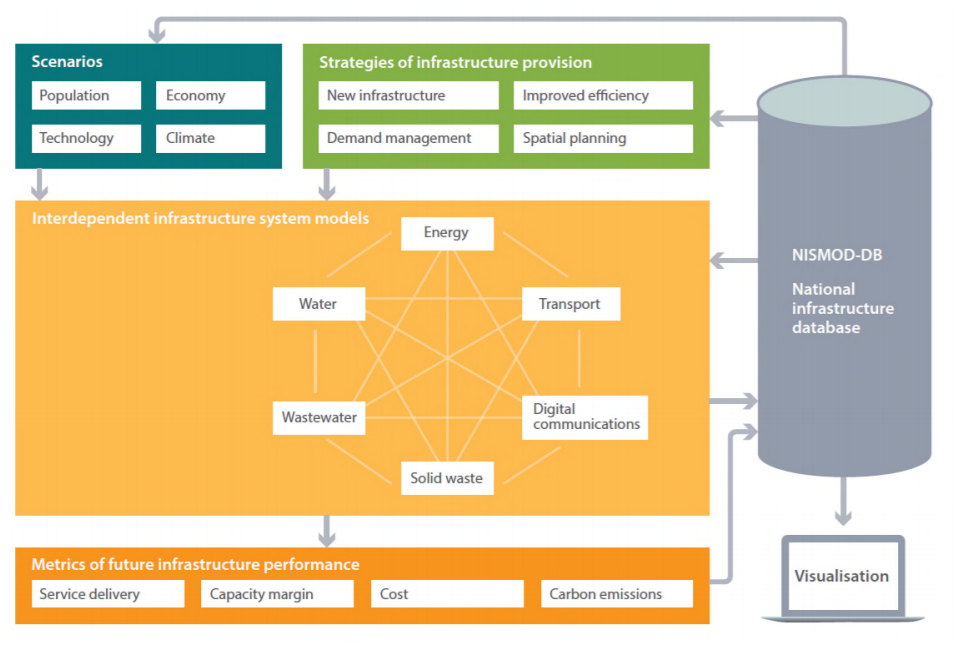
\includegraphics[width=1\textwidth]{./media/image14.png}
		\caption{The NISMOD system-of-systems model. ITRC-MISTRAL architecture\cite{3-12}}
	\end{Center}
\end{figure}


%%%%%%%%%%%%%%%%%%%% Figure/Image No: 14 Ends here %%%%%%%%%%%%%%%%%%%%

For this Master Thesis, I have used the digital communications model, available on GitHub \cite{3-04} under the MIT License, which allows «to deal with the Software without restriction, including without limitation the rights to use, copy, modify, merge, publish, distribute, sublicense, and/or sell copies of the Software». The code that was present in the repository when this thesis started is after the commit f80ce46d20deffd4d96a171e8030e98ce5d4ba02 \cite{3-09}.\par

In \cite{3-03}, Oughton, Edward et al. use the NISMOD project to quantify the uncertainty of future demand scenarios and measure the performance of different infrastructure interventions. This work uses the MINERVA (Mobile INfrastructuRe EVAluation) framework, which is under the NISMOD project, to test which infrastructure intervention strategies will be enough to meet the demand according to different demand growth rates.\par







\section{Original model}
%\addcontentsline{toc}{section}{Original model}
The following block diagram represents the structure of the project at the beginning of this Master Thesis. NISMOD stores all the information about regions and assets as well as projections of the evolution of the capacity and the demand in the UK and, given the preferred spectrum bands to use, the model can estimate how mobile network infrastructure will play out for different future scenarios.
%%%%%%%%%%%%%%%%%%%% Figure/Image No: 15 starts here %%%%%%%%%%%%%%%%%%%%
\begin{figure}[H]
	\begin{Center}
		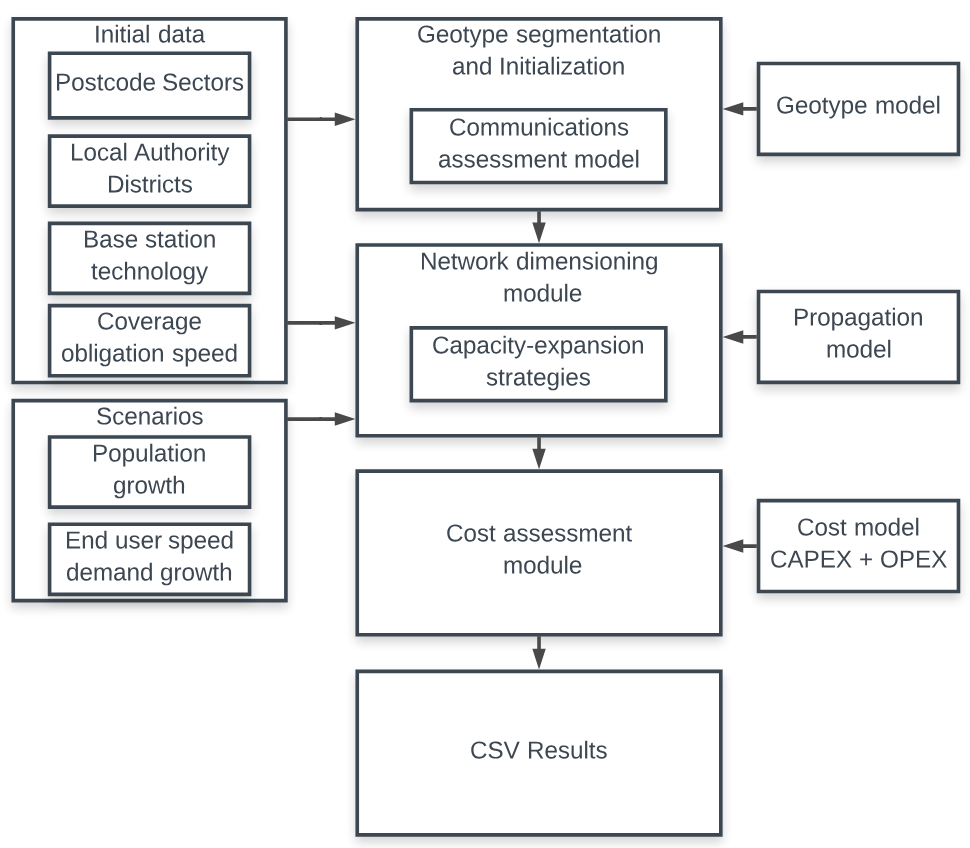
\includegraphics[width=0.95\textwidth]{./media/image15.png}
		\caption{NISMOD architecture\cite{3-03}}
	\end{Center}
\end{figure}
%%%%%%%%%%%%%%%%%%%% Figure/Image No: 15 Ends here %%%%%%%%%%%%%%%%%%%%
Population and end user speed demand projections are estimated using projection models, but only until 2030, since the accuracy of the projection decreases for longer periods. This project is capable of reporting costs and the capacity margin in each region at the end of each year. \par

\subsection{Initial data}
The project loads some scenario information at start time. This information is essential to define the environment where the simulations will take place. To assess the deployment of new assets, the code needs information about regions in which the country is divided, population and population density of the areas, and the initial assets present in the country at the beginning of the simulation. \par

\subsubsection*{Postcode Directory (PCD)}
%\addcontentsline{toc}{subsubsection}{Postcode Directory (PCD)}
It is the minimal geographical unit in the project and contains information about the population and the area in square meters. There are 8985 PCDs. The Cambridge model contains no information about Northern Ireland, and for this reason, results will only contain information about England, Scotland, and Wales.\par

\subsubsection*{Local Authority District (LAD)}
%\addcontentsline{toc}{subsubsection}{Local Authority District (LAD)}
A LAD is a group of PCDs. As there is no standard definition of LAD partitions, there are two types of LADs in the project: some which are used only for computational purposes and the ones used to generate the colour maps for the visualization module. There are 174 LADs when the information is represented on the maps.\  LADs are initialized with a list of PCDs that belong to the given LAD.\par


\subsubsection*{Initial assets}
%\addcontentsline{toc}{subsubsection}{Initial assets}
The code also loads all the information regarding assets that are already installed in the country. This is used to know the capacity of the network at the beginning and to be able to compute the capacity margin at the end of the year. For each asset, the model knows which technologies and frequencies it uses, in which PCD is, when was it built, and the spectrum bandwidth that it can use.\par


\subsubsection*{Investment}
%\addcontentsline{toc}{subsubsection}{Investment}
Investment of the telecommunications industry in the maintenance and development of the cellular networks is approximately £2 billion per year according to \cite{3-06}. In the model, this amount is divided proportionally to the market share. The market share of the telecom operator chosen for the tests is 30$\%$  which is the typical market share that the incumbent telecom operator has in a 4 telecom operators scenario, such as Spanish and British scenarios.\par


\subsubsection*{Coverage obligation}
%\addcontentsline{toc}{subsubsection}{Coverage obligation}
This version of the code has a really simple way of leading with coverage obligations. It fixes a threshold for coverage obligations, which is predefined as 10 Mbps/km\textsuperscript{2} independently of the population of the postcode which is not how Ofcom sets coverage obligations.\par


\subsubsection*{Simulation options}
%\addcontentsline{toc}{subsubsection}{Simulation options}
The model allows choosing between several scenarios to test the influence that each parameter has on the outputs. All of the parameters are explained in higher detail in the following sections, but a shorter description is:\par

\begin{itemize}
	\item \textit{pop\_scenario} which represent the rate at which the population growths. There are four options: static, low, medium, high. It is explained in section C. Scenario projections.\par

	\item \textit{throughput\_scenario} which represents how the demand per user growths over time. There are three options: low, medium, high. It is explained in section C. Scenario projections.\par

	\item \textit{intervention\_strategy }which represent the specific interventions that are allowed in this run. There are four options: Minimum intervention, Spectrum integration strategy, small cells strategy, and Hybrid strategy. It is explained in section D. Network dimensioning module.\par
\end{itemize}

\subsection{Geotype segmentation and initialization}
This module takes all the information loaded at start time and computes MINERVA, the \textit{«Mobile INfrastructuRe EVAluation framework». }MINERVA is an object that contains the current information about all the regions and updates it when there are changes in the population information or when a new asset is built. \par

\subsubsection*{Geotype model}
%\addcontentsline{toc}{subsubsection}{Geotype model}
PCDs are segmented into geotypes when they are added to the CCAM. Geotypes are used to perform a more granular analysis of the rollout and represent the key supply-side variables that affect the rollout costs. This project uses the categorization that Analysis Mason used in \cite{3-011} for Ofcom. The module segments areas with similar characteristics, such as similar population density, and classify the regions into three main types: urban, suburban and rural. Each main type is then subdivided into one or more geotypes, and the full picture of the UK with the distribution of the geotypes around the country is shown in the following figure:
%%%%%%%%%%%%%%%%%%%% Figure/Image No: 16 starts here %%%%%%%%%%%%%%%%%%%%
\begin{figure}[H]
	\begin{Center}
		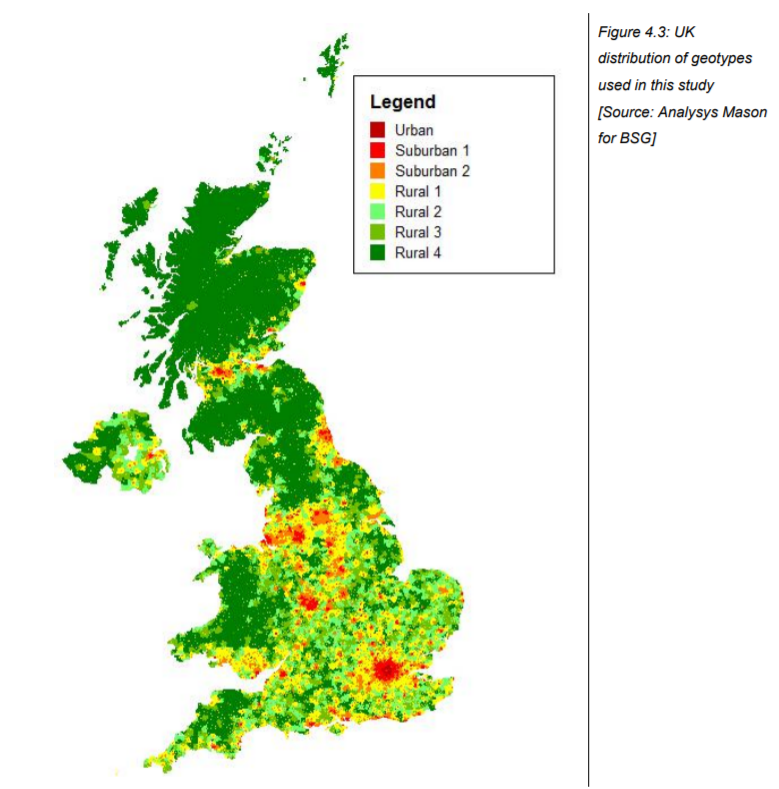
\includegraphics[width=0.7\textwidth]{./media/image16.png}
		\caption{Geotypes in the UK. Analysis Mason\cite{3-11}}
	\end{Center}
\end{figure}
%%%%%%%%%%%%%%%%%%%% Figure/Image No: 16 Ends here %%%%%%%%%%%%%%%%%%%%
For the sake of simplicity, NISMOD divides regions into the three main geotypes: Urban, suburban and rural. (I) When the population density is at least 7,959 inhabitants per square meter, the area is considered of geotype Urban. This occurs approximately on 0.2$\%$  of the area of Britain and 8.3$\%$  of the population. (II) The second type is Suburban and is for regions with population density from 782 to 7,958 inhabitants per square meter. This region covers 7$\%$  of the area and 61$\%$  of the population. (III) Finally, the rural area is for regions with lower population densities and covers 92$\%$  of Britain’s size, but just 29$\%$  of the population.\par

Despite some PCDs being considerably homogeneous, most of them contain some parts that could be categorized as urban, suburban and rural. We do not have such detailed database to perform that analysis and, therefore, some areas could be miscategorized. For example, a PCD with 4,000 inhabitants and 1km\textsuperscript{2} would be considered suburban, but if the population is living in just the 50$\%$  of the area, the site density of the urban part is 8,000, so it would be categorized as 50$\%$  urban and 50$\%$  rural (If nobody lives in this part). This issue cannot be resolved with the current data of the model because the percentage of the area where inhabitants live over the total varies significantly in each PCD.
%%%%%%%%%%%%%%%%%%%% Figure/Image No: 17 starts here %%%%%%%%%%%%%%%%%%%%
\begin{figure}[H]
	\begin{Center}
		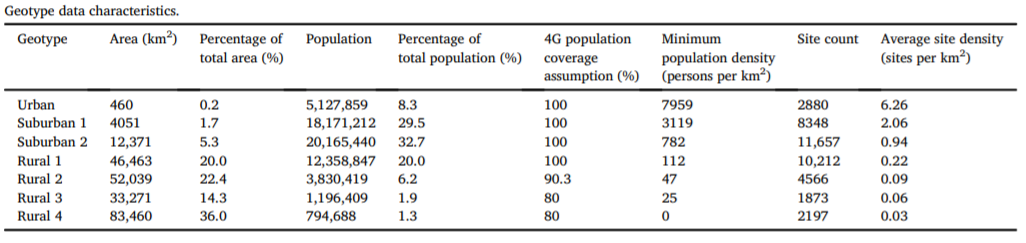
\includegraphics[width=1.1\textwidth]{./media/image17.png}
		\caption{Geotypes data characteristics. Edward J. Oughton and Zoraida Frias\cite{3-03}}
	\end{Center}
\end{figure}
%%%%%%%%%%%%%%%%%%%% Figure/Image No: 17 Ends here %%%%%%%%%%%%%%%%%%%%
\subsection{Scenario projections}
Two main projections are used in this project: the estimation of the growth of the population and the calculation of the demand for download speed from 2020 to 2030. Two are the reasons why 2030 is the last year of the projections: (I) Population trend may vary a lot in the years to come - check the following link with population projections prepared by the United Nations \cite{3-07} – so it makes no sense to predict data for more than 10 years. End-user speed may vary even more drastically than population. (II) Telecommunication technologies evolve quite fast and considering that there will not appear new technologies in more than 10 years is a conservative planning approach that may not occur.
%%%%%%%%%%%%%%%%%%%% Figure/Image No: 18 starts here %%%%%%%%%%%%%%%%%%%%
\begin{figure}[H]
	\begin{Center}
		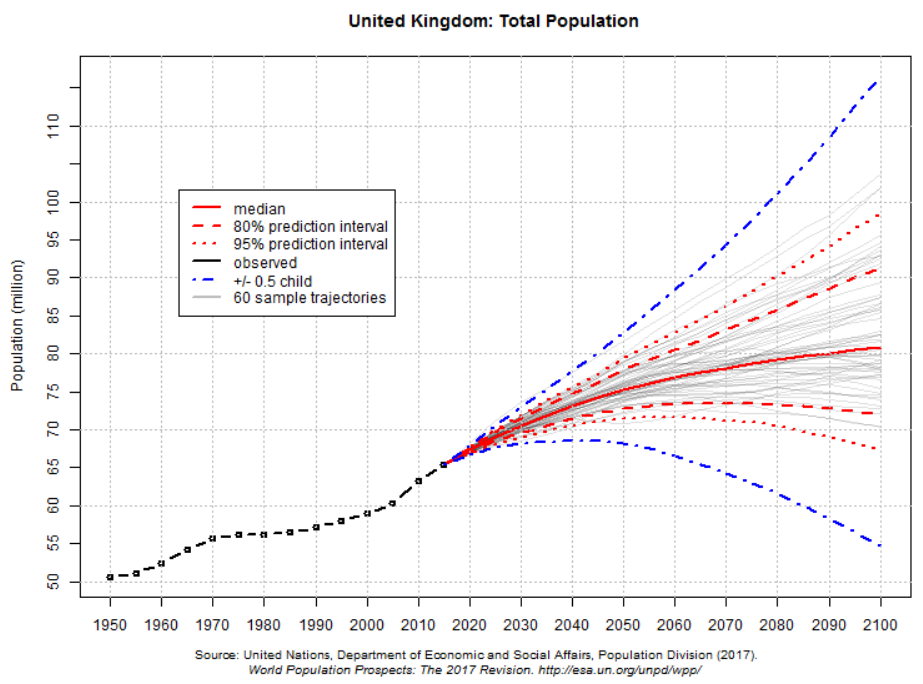
\includegraphics[width=0.8\textwidth]{./media/image18.png}
		\caption{Projections of the population in the UK. United Nations\cite{3-13}}
	\end{Center}
\end{figure}
%%%%%%%%%%%%%%%%%%%% Figure/Image No: 18 Ends here %%%%%%%%%%%%%%%%%%%%
\subsubsection*{Population projections}
%\addcontentsline{toc}{subsubsection}{Population projections}
Data of the population of each PCD has been taken from the UK Census. As Scotland has not published more population data since 2011, the data used in the project is taken from the 2011 Census and then aggregated for each PCD. The population growth model is in the NISMOD GitHub, but outside the digital\_comms repository, as it is used for all the Interdependent infrastructure system models. The repository \cite{3-08} allows creating several projections depending on the fertility, life expectancy, migration, future EU migration and other factors. In this thesis, the population for the following years is modelled according to four different approximations depending on the growing rate forecasted: $``$Static$"$ , $``$low$"$ , $``$medium$"$  and $``$high$"$.



%%%%%%%%%%%%%%%%%%%% Figure/Image No: 19 starts here %%%%%%%%%%%%%%%%%%%%

\begin{figure}[H]
	\begin{Center}
		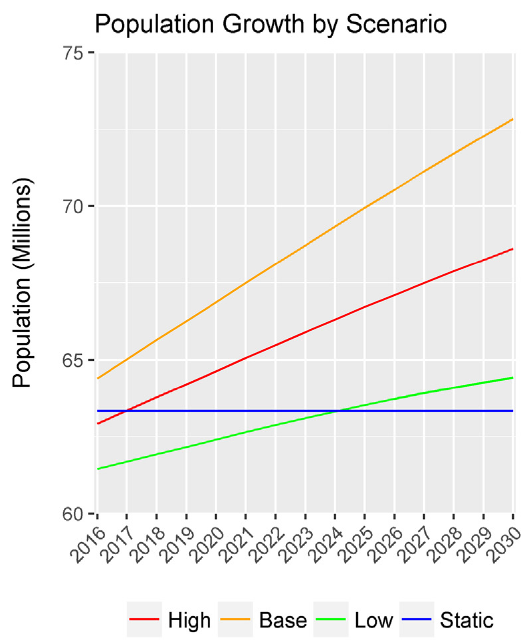
\includegraphics[width=0.60\textwidth]{./media/image19.png}
		\caption{Population scenarios. NISMOD\cite{3-07}}
	\end{Center}
\end{figure}
%%%%%%%%%%%%%%%%%%%% Figure/Image No: 19 Ends here %%%%%%%%%%%%%%%%%%%%
For a deeper explanation, please refer to the following paper \cite{3-03}.

\subsubsection*{End-user speed projections}
%\addcontentsline{toc}{subsubsection}{End-user speed projections}
Demand in each PCD is part of the outputs of this project, but results may vary depending on the model used. Demand projections are estimated in data consumption per month and per user. As in the population projections, the demand growth rate is not included in the source code, but the model is perfectly parametrized, so new estimations can be added. \par

The Cisco VNI white paper \cite{3-08} has been used to estimate the end-user speed demand. Their report for 2016-2021 states that: «Mobile network connection speeds will increase threefold by 2021. The average mobile network connection speed (6.8 Mbps in 2016) will reach 20.4 megabits per second (Mbps) by 2021» and «The average smartphone will generate 6.8 GB of traffic per month by 2021, a fourfold increase over the 2016 average of 1.6 GB per month. By 2021, aggregate smartphone traffic will be seven times greater than it is today, with a CAGR of 48 per cent».



%%%%%%%%%%%%%%%%%%%% Figure/Image No: 20 starts here %%%%%%%%%%%%%%%%%%%%

\begin{figure}[H]
	\begin{Center}
		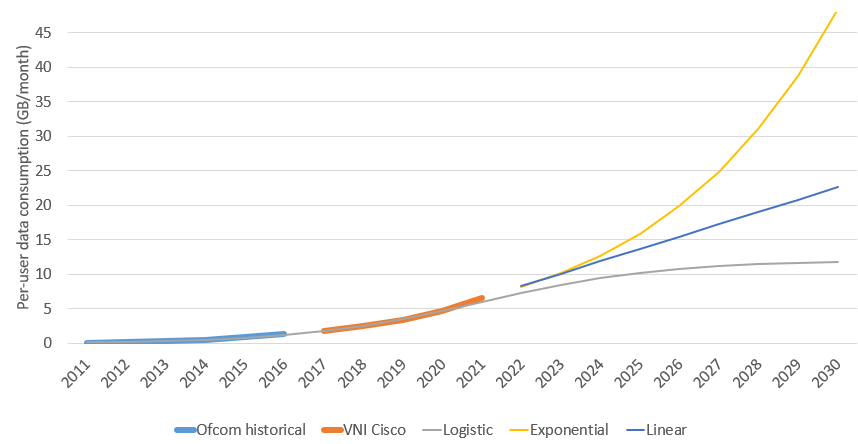
\includegraphics[width=0.9\textwidth]{./media/image20.png}
		\caption{End-user speed demand in the busy hour projections. NISMOD\cite{3-07}}
	\end{Center}
\end{figure}


%%%%%%%%%%%%%%%%%%%% Figure/Image No: 20 Ends here %%%%%%%%%%%%%%%%%%%%


This thesis uses three different models to estimate the variation of the demand across the years:\par

\begin{itemize}
	\item Logistic approximation which in the visualization model is named as $``$low$"$ . This scenario is the $``$worst$"$  for the 5G adoption, as it would mean that no killer app or data consumption model has appeared to change the way people use broadband data services.\par

	\item Linear evolution which is named $``$medium$"$  in the visualization model.\par

	\item Exponential evolution of the data consumption at 25$\%$  Compound annual growth rate over 2021-2030 which is named as $``$high$"$ .
\end{itemize}

\vspace{\baselineskip}


%%%%%%%%%%%%%%%%%%%% Figure/Image No: 21 starts here %%%%%%%%%%%%%%%%%%%%

\begin{figure}[H]
	\begin{Center}
		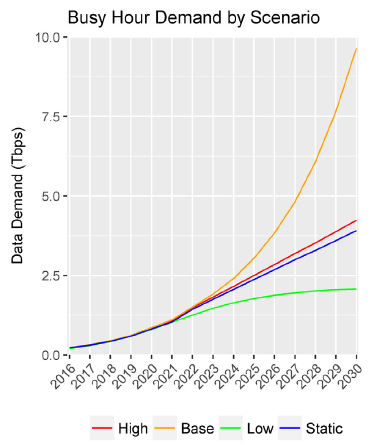
\includegraphics[width=0.60\textwidth]{./media/image21.png}
		\caption{End-user speed demand in the busy hour projections. NISMOD\cite{3-07}}
	\end{Center}
\end{figure}


%%%%%%%%%%%%%%%%%%%% Figure/Image No: 21 Ends here %%%%%%%%%%%%%%%%%%%%

Once the models are introduced into the program, the demand is transformed from GB per month per user to Mbps per user in the busy hour. The formula used is:\par
\begin{multline*} Demand\_in\_mbps = Demand\_in\_GB \\ $\ast$ 1024 $\ast$ 8 $\ast$ percentage / 30 / 3600 \end{multline}

where percentage is the percentage of the traffic in the busy hour. It is estimated as 7.5$\%$ of the total traffic of the day.\par



\subsection{Network dimensioning module}
For each year, as long as there is enough budget for more investments, the project checks the PCDs in order, from more densely populated areas to less, looking for PCDs where the demand is higher than the capacity installed. This module is called once per year and PCD and triggers the suggest\_intervention function every time there is a lack of capacity in a PCD in the given year. This function checks the intervention options allowed in the PCD and builds the assets that the PCD needs to reach the capacity.\par

The model uses the capacity lookup table to calculate the capacity installed and the extra capacity provided by the new assets. The model has also several predefined interventions which are basically one per technology and capacity-expansion strategies, which are the set of interventions that are allowed in each simulation.\par

\subsubsection*{Propagation model}
%\addcontentsline{toc}{subsubsection}{Propagation model}
The propagation model is a set of curves that estimate the capacity per area unit of the PCD depending on the site density (only considering assets that have the same frequency and technology), the frequency, bandwidth and technology and the geotype of the given PCD \cite{3-09}.\par

Each capacity curve is calculated using several cell parameters, such as the macrocellular layout, the frequency reuse factor, the cell-edge, the overbooking factor, etc. A comprehensive study of how all these factors influence in the network capacity can be checked in \cite{3-10}. The following table represents all the parameters considered in the estimations:



%%%%%%%%%%%%%%%%%%%% Figure/Image No: 22 starts here %%%%%%%%%%%%%%%%%%%%

\begin{figure}[H]
	\begin{Center}
		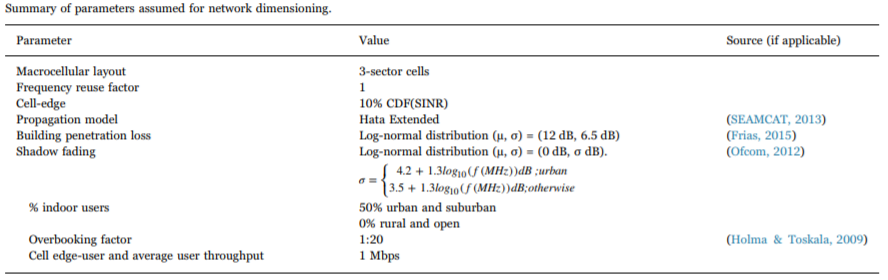
\includegraphics[width=1.05\textwidth]{./media/image22.png}
		\caption{Network dimensioning parameters. Zoraida Frias\cite{3-14}}
	\end{Center}
\end{figure}


%%%%%%%%%%%%%%%%%%%% Figure/Image No: 22 Ends here %%%%%%%%%%%%%%%%%%%%

%\vspace{\baselineskip}
%\textbf{Aquí hay que hablar sobre las tablas de propagación:}\par
%
%
%
%%%%%%%%%%%%%%%%%%%%% Figure/Image No: 23 starts here %%%%%%%%%%%%%%%%%%%%
%
%\begin{figure}[H]
	%\begin{Center}
		%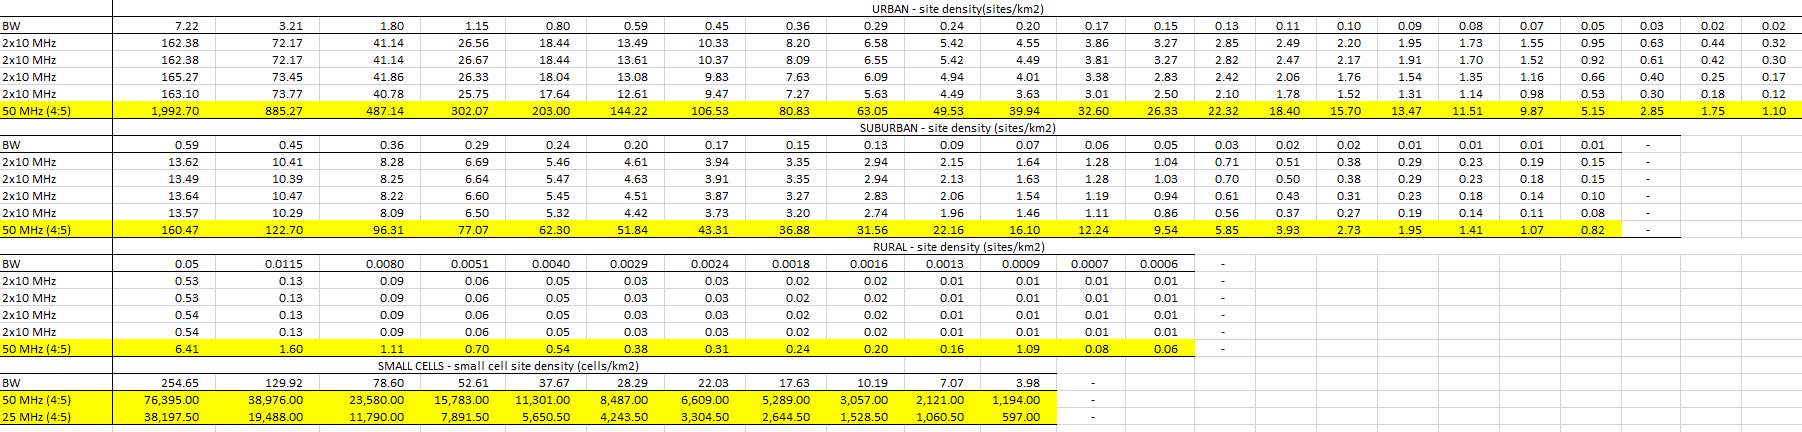
\includegraphics[width=6.5in,height=1.56in]{./media/image23.png}
		%\caption{}
	%\end{Center}
%\end{figure}
%
%
%%%%%%%%%%%%%%%%%%%%% Figure/Image No: 23 Ends here %%%%%%%%%%%%%%%%%%%%
%
%\textbf{ }\par
%
%\textbf{De alguna manera hay que explicar que las regiones rurales tienen una capacidad máxima menor y cosas así.}\par

\subsubsection*{Interventions}
%\addcontentsline{toc}{subsubsection}{Interventions}
There are four intervention types defined in the Network Dimensioning model. Each of them implies normally the usage of one specific technology but choosing one does not directly prevent the telecom operator from using the rest. The possible interventions in the original model where:\par

\begin{itemize}
	\item $``$Upgrade site to LTE$"$ : This intervention is available for every already built asset that has only 2G and 3G. When it is possible to build more than one intervention, this one has a higher priority than the rest. This intervention is a combination of building: (I) 800 MHz carrier with LTE technology and 2x10 MHz (II) 2600 MHz carrier with LTE technology and 2x10 MHz in the same place were the original asset was.\par

	\item $``$Build 700 MHz carrier$"$ : This intervention is only possible in those sites that do not emit in 700 MHz yet, but has already performed the upgrade to LTE intervention. It can be built only from 2020 onwards since this is the carrier that will be allocated to telecommunications in most European countries after the second digital dividend. This intervention builds a 700 MHz carrier of 2x10 MHz in the same place where the original asset was.\par

	\item $``$Build 3500 MHz carrier$"$ : This intervention is only possible in those sites that do not emit in 3500 MHz yet, but has already performed the upgrade to LTE intervention. As the 700 MHz band, it can be built only from 2020 onwards because it is the 3.4 GHz band that was awarded in April 2018 with the aim of using it for 5G services. This intervention builds a 3500 MHz carrier of 50 MHz in the same place where the original asset was.\par

	\item $``$Build a small cell$"$ : This intervention builds a new site in a place that does not necessarily need to have a previous macrocell asset built. It builds a small cell asset with 5G technology, in the band of 3700 MHz and with a bandwidth of 2x25 MHz. This type of assets cannot be built until 2020 for the same reason as the previous ones.\par

It is worth noting that 900 MHz, 1800 MHz, and 2100 MHz are excluded from the current analysis as legacy networks operate on that spectrum and there is no evidence to suggest that this bands will be refarmed to 5G technologies in the midterm, at least before 2030 which is the last year of study.\par


\end{itemize}
\subsubsection*{Capacity-expansion strategies}
%\addcontentsline{toc}{subsubsection}{Capacity-expansion strategies}
Not all the situations allow building any type of intervention because maybe a specific band is not allocated for broadband services in a given country or the telecom operator tested has no spectrum allocated in this band. Capacity-expansion strategies allow creating the set of interventions that will be available in each test.\par

This mechanism also simplifies the analysis for telecom operators, since they can simulate the effects that bidding for more bandwidth in a new band will take into their budget. And even for policymakers, because they will be able to quantify the importance of a given spectrum for a specific telecom operator and the amount of money that they would be willing to pay for it. \par

Four types of strategies have been defined in this model:\par



%%%%%%%%%%%%%%%%%%%% Table No: 6 starts here %%%%%%%%%%%%%%%%%%%%


\begin{table}[H]
 			\centering
\begin{tabular}{p{1.35in}p{3.92in}}
\hline
%row no:1
\multicolumn{1}{|p{1.35in}}{\Centering \textbf{Strategy name}} & 
\multicolumn{1}{|p{3.92in}|}{\Centering \textbf{Description}} \\
\hhline{--}
%row no:2
\multicolumn{1}{|p{1.35in}}{\Centering Minimum intervention} & 
\multicolumn{1}{|p{3.92in}|}{This strategy operates and maintains existing network and does not deploy new assets in any frequency band.} \\
\hhline{--}
%row no:3
\multicolumn{1}{|p{1.35in}}{\Centering 700MHz spectrum integration} & 
\multicolumn{1}{|p{3.92in}|}{Upgrade to LTE if not available (800 MHz and 2600 MHz). \par Integrate spectrum in the 700 MHz band.} \\
\hhline{--}
%row no:4
\multicolumn{1}{|p{1.35in}}{\Centering Spectrum integration} & 
\multicolumn{1}{|p{3.92in}|}{Upgrade to LTE if not available (800 MHz and 2600 MHz). \par Integrate all another spectrum on the brownfield microcellular network (700 and 3500 MHz).} \\
\hhline{--}
%row no:5
\multicolumn{1}{|p{1.35in}}{\Centering Small cells strategy} & 
\multicolumn{1}{|p{3.92in}|}{Upgrade to LTE if not available (800 MHz and 2600 MHz). \par Deploy a greenfield small cell layer operating in TDD at 3700 MHz.} \\
\hhline{--}
%row no:6
\multicolumn{1}{|p{1.35in}}{\Centering Hybrid strategy} & 
\multicolumn{1}{|p{3.92in}|}{Upgrade to LTE if not available (800 MHz and 2600 MHz). \par Integrate all another spectrum on the brownfield microcellular network (700 and 3500 MHz). \par Deploy a greenfield small cell layer operating in TDD at 3700 MHz.} \\
\hhline{--}

\end{tabular}
\caption{Capacity expansion strategies. NISMOD}
 \end{table}


%%%%%%%%%%%%%%%%%%%% Table No: 6 ends here %%%%%%%%%%%%%%%%%%%%


\vspace{\baselineskip}
\subsection{Cost assessment module}
Every time the network dimensioning module builds a new intervention, the cost assessment module is triggered to store the type of intervention, the year and how much does this specific intervention cost. This way the model knows how much has been spent in the current year and if there is enough budget for more interventions. The cost assessment module uses a cost model which is explained in higher detail in the following paper \cite{3-03}.\par

\subsubsection*{Cost model}
%\addcontentsline{toc}{subsubsection}{Cost model}
The cost of each intervention can be calculated using the following formula:\par

 \[ Total\_cost\_of\_an\_intervention = CAPEX + OPEX \] \par

The Capital Expenditures (CAPEX) of the $``$upgrade to LTE$"$  intervention is the cost of deploying a multicarrier BS (£40,900) plus the cost of the civil works (£18,000). As the multicarrier base station lifetime is estimated at 10 years and the original project runs from 2017, two multicarrier base stations are needed. The Operational Expenditures (OPEX) of the $``$upgrade to LTE$"$  intervention is £3,898 per year. To aggregate all of these costs, the present value of the future cash flow has been calculated using a discount rate of 3.5$\%$  and the total cost is estimated at £142,446.\par

The cost calculated for the strategies $``$700 MHz integration$"$  and $``$3500 MHz integration$"$  is the same because these strategies can only be undertaken if there is an existing LTE base station in the list of assets. Therefore, the cost of deploying a multicarrier base station (£40,900) is reduced to only installing an additional carrier on the current base station, which is only £15,000. The OPEX is also reduced to £1,800 and therefore, the total cost discounted to the present value is £50,917.\par

Lastly, the cost of the small cell strategy is calculated using the CAPEX plus OPEX formula, but in this case, the small cell is expected to have only 5 years of lifetime, so 4 small cells have to be built. Each small cell equipment is £2,500 and the civil works (which are needed just the first time) are £13,300. Opex is calculated as the OPEX of the small cell equipment (£350) plus the £1,000 of backhaul OPEX. The total amount that this intervention costs discounted to the present value is £40,220.\par

A summary of the costs of each asset is made based on the following table that was extracted from \cite{3-10}:



%%%%%%%%%%%%%%%%%%%% Figure/Image No: 24 starts here %%%%%%%%%%%%%%%%%%%%

\begin{figure}[H]
	\begin{Center}
		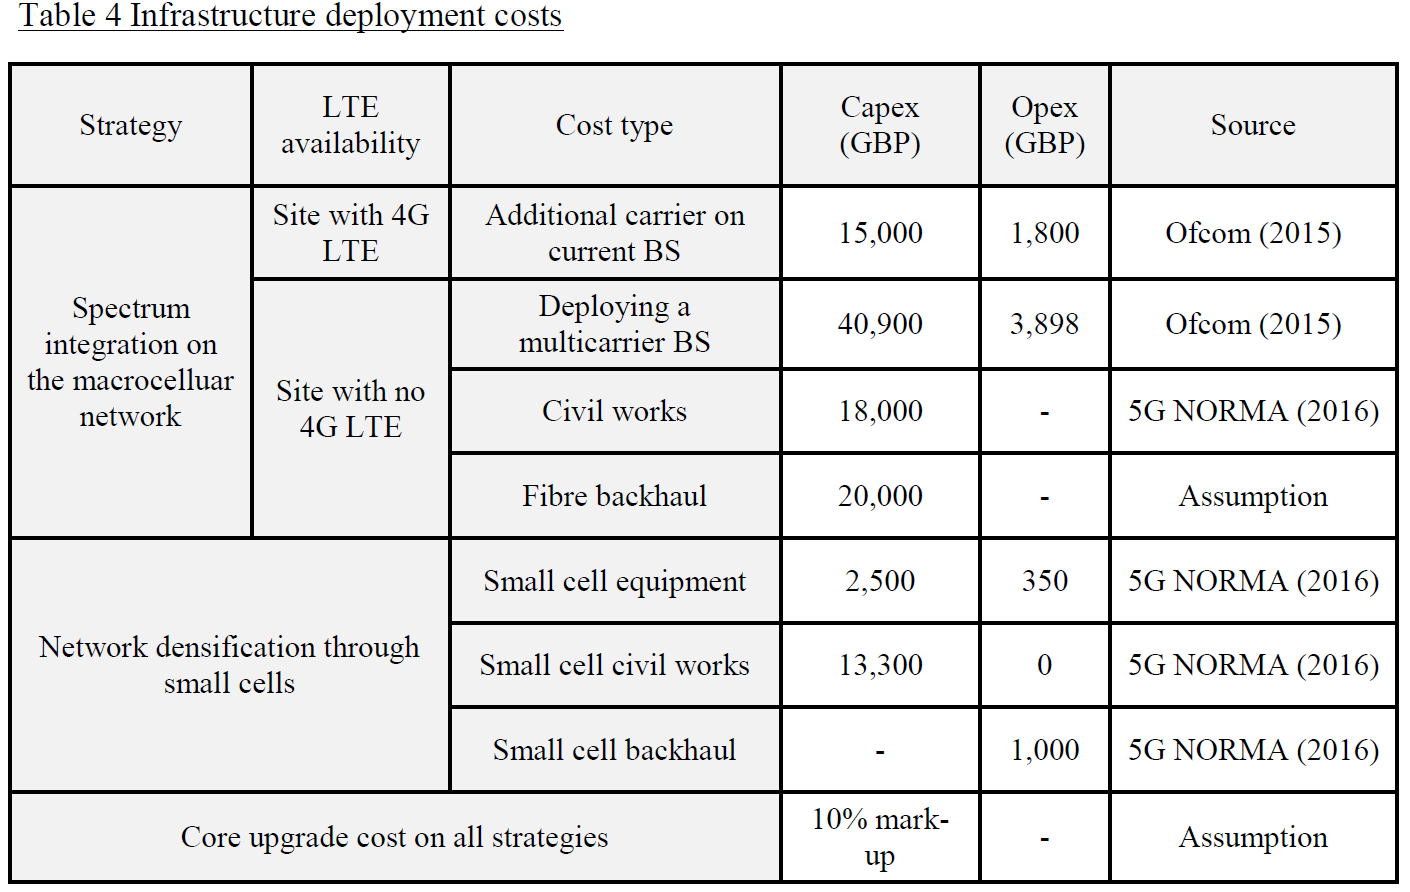
\includegraphics[width=0.95\textwidth]{./media/image24.png}
		\caption{Infrastructure deployment costs. NISMOD\cite{3-10}}
	\end{Center}
\end{figure}


%%%%%%%%%%%%%%%%%%%% Figure/Image No: 24 Ends here %%%%%%%%%%%%%%%%%%%%


\subsection{Model results}
This section describes the outcomes of the original model. The outputs are grouped in three types of .csv files in the outputs folder. Each of them provides the following information:\par

\begin{itemize}
	\item Decisions.csv provides information about the assets that were built in the simulation and their related information: in which year, in which PCD and specific asset (all the interventions, except small cells, are built at existing sites), the type and technology of the installation and the frequency and bandwidth.\par

	\item Metrics.csv and pcd\_metrics.csv provide information about the deployment situation after the network dimensioning module algorithm has been run for each year. The metrics.csv file gives information of the LADs and the pcd\_metrics.csv file gives information of the PCDs. The information of each PCD and LAD is total demand per km\textsuperscript{2}, total capacity per km\textsuperscript{2}, capacity deficit per km\textsuperscript{2}, population and population density.\par

	\item Spend.csv provides information about the interventions built and the cost that their cost.\par

This is all the information that the model outputs provide. The rest of the information has to be calculated or represented using external tools that are not included.\par


\end{itemize}
\subsubsection*{Timeframe}
%\addcontentsline{toc}{subsubsection}{Timeframe}
It is possible to know when the model decides that no more assets are needed to satisfy the data demand and the coverage obligations set by i.e. a policymaker, just by aggregating all the expenses per year and checking in which year the total sum is less than the available budget.\par

\subsubsection*{Capacity}
%\addcontentsline{toc}{subsubsection}{Capacity}
Capacity in each PCD is measured per km\textsuperscript{2} and is the result of aggregating the capacity provided by all the assets in each PCD. Representing the value of the capacity results in a figure that is not so useful, because the values in the y-axis do not have a specific shape, not as demand and capacity margin figures. For the sake of consistency and to explain the shape of the capacity margin, it can be checked below:



%%%%%%%%%%%%%%%%%%%% Figure/Image No: 25 starts here %%%%%%%%%%%%%%%%%%%%

\begin{figure}[H]
	\begin{Center}
		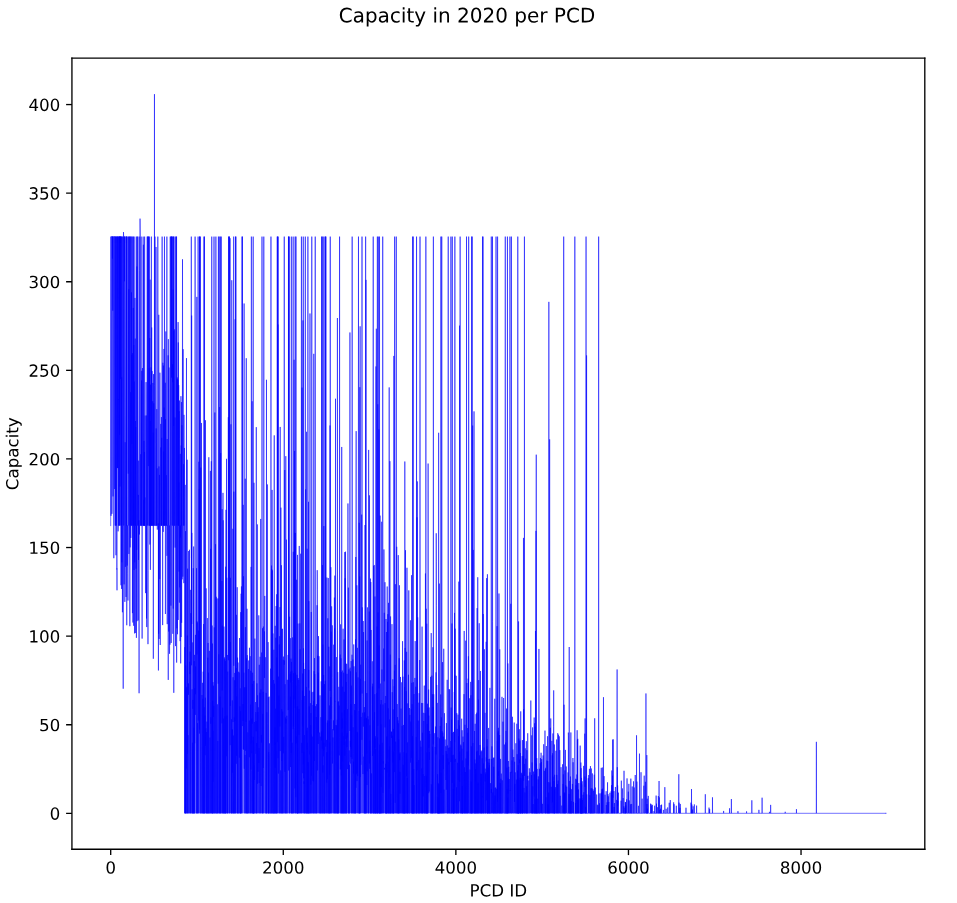
\includegraphics[width=0.95\textwidth]{./media/image25.png}
		\caption{Capacity in 2020 per PCD. Source: Author}
	\end{Center}
\end{figure}


%%%%%%%%%%%%%%%%%%%% Figure/Image No: 25 Ends here %%%%%%%%%%%%%%%%%%%%


\subsubsection*{Demand}
%\addcontentsline{toc}{subsubsection}{Demand}
The demand in each PCD is also measured per km\textsuperscript{2} and is calculated according to the rules explained in the End-user speed projections section. The resulting demand is obtained by multiplying the potential users by the demand per user and an overbooking factor that represent that not all the users are demanding network resources simultaneously.\par

 \[ Demand = users\ast demand \_ per \_ user \ast overbooking \_ factor / area \] \par

where:\par

\begin{itemize}
	\item \textit{users} is estimated multiplying the whole population of the PCD by the mobile broadband services penetration (estimated in 80$\%$ ) and by the market share of the telecom operator (in this case is 30$\%$ ).\par

	\item The \textit{overbooking\_factor} is set to 50.\par

	\item The \textit{area} is the area of each PCD.\par

	\item \textit{Demand\_per\_user} is obtained from the end-user speed demand chart and then converted from demand in GB/month to Mbps/user using the following formula:\par
\end{itemize}
\begin{Center}
\begin{multline*}
Demand \_ in \_ mbps =Demand \_ in \_ GB \ \ast \ 1024 \ \ast 8 \ast \\
 Traffic \_ in \_ busy \_ hour \ / 30 \ / 3600
\end{multline}
\end{Center}\par

Hence, graphically, \textit{Demand\_in\_Mbps} is the result of multiplying the area by the demand per user (which has one of the given functions in the projection section) by several factors and that is why the demand has the shape in the following figure:



%%%%%%%%%%%%%%%%%%%% Figure/Image No: 26 starts here %%%%%%%%%%%%%%%%%%%%

\begin{figure}[H]
	\begin{Center}
		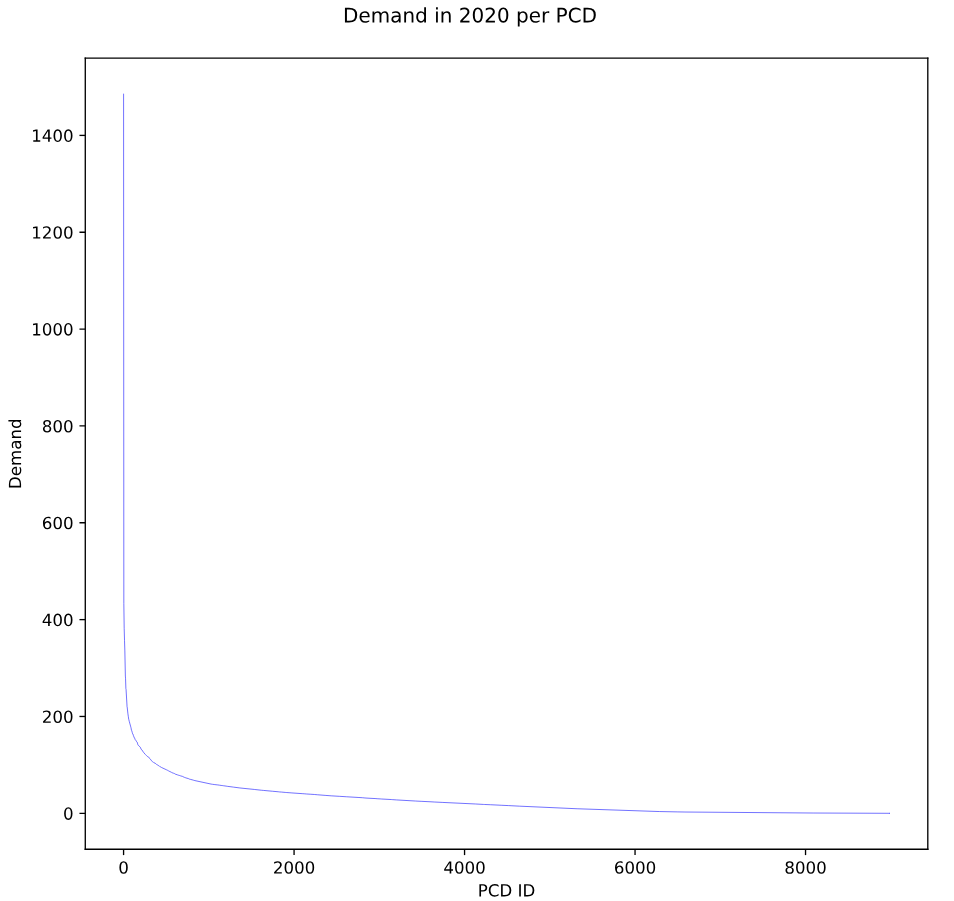
\includegraphics[width=0.95\textwidth]{./media/image26.png}
		\caption{Demand in 2020 per PCD. Source: Author}
	\end{Center}
\end{figure}


%%%%%%%%%%%%%%%%%%%% Figure/Image No: 26 Ends here %%%%%%%%%%%%%%%%%%%%



\subsubsection*{Capacity margin}
%\addcontentsline{toc}{subsubsection}{Capacity margin}
The capacity margin for a given PCD is the result of the capacity minus the demand and is measured in Mbps/km\textsuperscript{2}. In the PCDs graph, the capacity margin function is just the result of subtracting the demand function from the capacity one. Negative values represent a capacity deficit. This is the formula to calculate the capacity margin:\par

 \[ Capacity\_ margin  \left( Mbps/km^{2} \right) = Capacity  \left( Mbps/km^{2} \right)  - Demand  \left( Mbps/km^{2} \right)  \] 

%%%%%%%%%%%%%%%%%%%% Figure/Image No: 27 starts here %%%%%%%%%%%%%%%%%%%%

\begin{figure}[H]
	\begin{Center}
		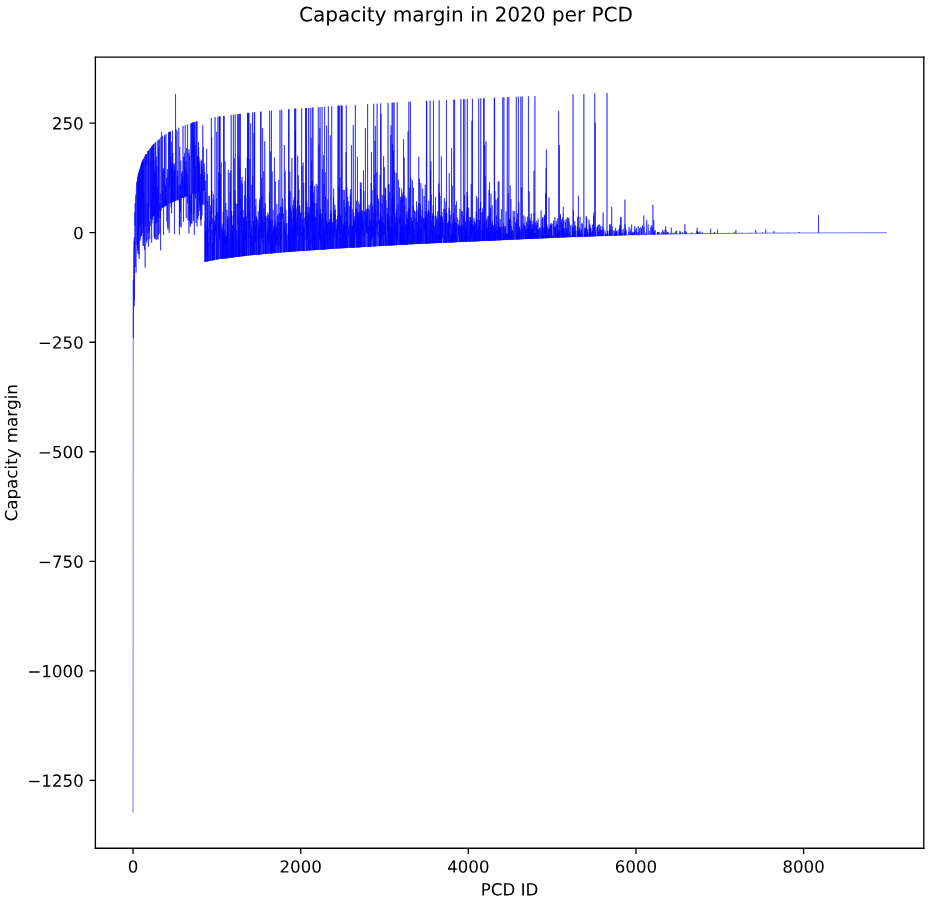
\includegraphics[width=0.95\textwidth]{./media/image27.png}
		\caption{Capacity margin in 2020 per PCD. Source: Author}
	\end{Center}
\end{figure}


%%%%%%%%%%%%%%%%%%%% Figure/Image No: 27 Ends here %%%%%%%%%%%%%%%%%%%%

\subsubsection*{Cost and capacity margin}
%\addcontentsline{toc}{subsubsection}{Cost and capacity margin}
The capacity margin is as important as costs in the model because one cannot show the whole picture without the other. A given cost is better or worst depending on if it has raised more or less the capacity margin, which is a measure of effectiveness. This fact shows the differences between urban, suburban and rural areas since rural area investments are not so efficient rising the capacity margin as investments in urban areas.\par

When comparing results from different scenarios and capacity-expansion strategies, for similar costs, better capacity margins imply better strategies a priori. And for similar capacity margins, fewer costs imply better strategies a priori.\par

When neither the capacity margin and the cost is similar, the decision of which strategy is better depends on aspects which are out of the scope of the digital comms project, because they are related to the interest of the government and stakeholders to have a universal access to broadband services in the country, the macroeconomic situation of the country, etc.\par


















 %%%%%%%%%%%%  Starting New Page here %%%%%%%%%%%%%%
%\vspace{\baselineskip}
\section{Contribution to the project}
%\addcontentsline{toc}{subsection}{Contribution to the project}
The following diagram shows the previous state of the project and the green boxes represent the modules that have been further developed in this Master Thesis. The first contribution to the project, and the one that enabled the rest of them was the creation of a data management structure to store some of the environment options and, more importantly, to store the results and measurements of the different iterations of the project.\par

After setting the base to modify the project, a detailed structure was created to set coverage obligations. Previously, users could only set a fixed end-user speed as a coverage obligation. Now, users can create coverage obligation options or use the predefined ones, which are as complex as the ones requested in reality by countries like Spain and the UK.\par

In addition, due to the expected importance of the 700 MHz band, a new intervention and a capacity expansion strategy have been defined to test the possibility of densifying the telecommunication network in a similar way to the small cell network. Thus, it is now possible to add more 700 MHz sites than the total amount of LTE and 2G/3G sites that are already installed.\par

The visualisation module is another relevant contribution to the project. When the thesis started, the project was only able to provide information in csv files. This information could be enough, but it was difficult to read without using data analysis tools since there are almost 9,000 PCDs. For this reason, the visualization module was created as a common hub to select which specific data and in which visualization sub-module should the data be processed.\par

The current version of the project allows one to output the data in csv, graphs, and coloured maps format. It also allows creating gifs that show the evolution of a specific parameter over the simulation time. Maps represent results at a LAD accuracy level because it is easier to see the differences and similarities between regions and how the network capacity evolves across the country. To visualise aggregate data that cannot be added directly, such as the percentage of population covered, the values of each PCD are weighted by the population of each PCD.\par

The project has two modules called maps.py and plots.py that have some predefined types of plots to print all the graphs and maps of this Thesis. These functions can be called with other parameters and data, so it is easy to plot other measures than the ones that are currently shown.\par

In the following chapter, all these contributions will be explained in more detail.



%%%%%%%%%%%%%%%%%%%% Figure/Image No: 28 starts here %%%%%%%%%%%%%%%%%%%%

\begin{figure}[H]
	\begin{Center}
		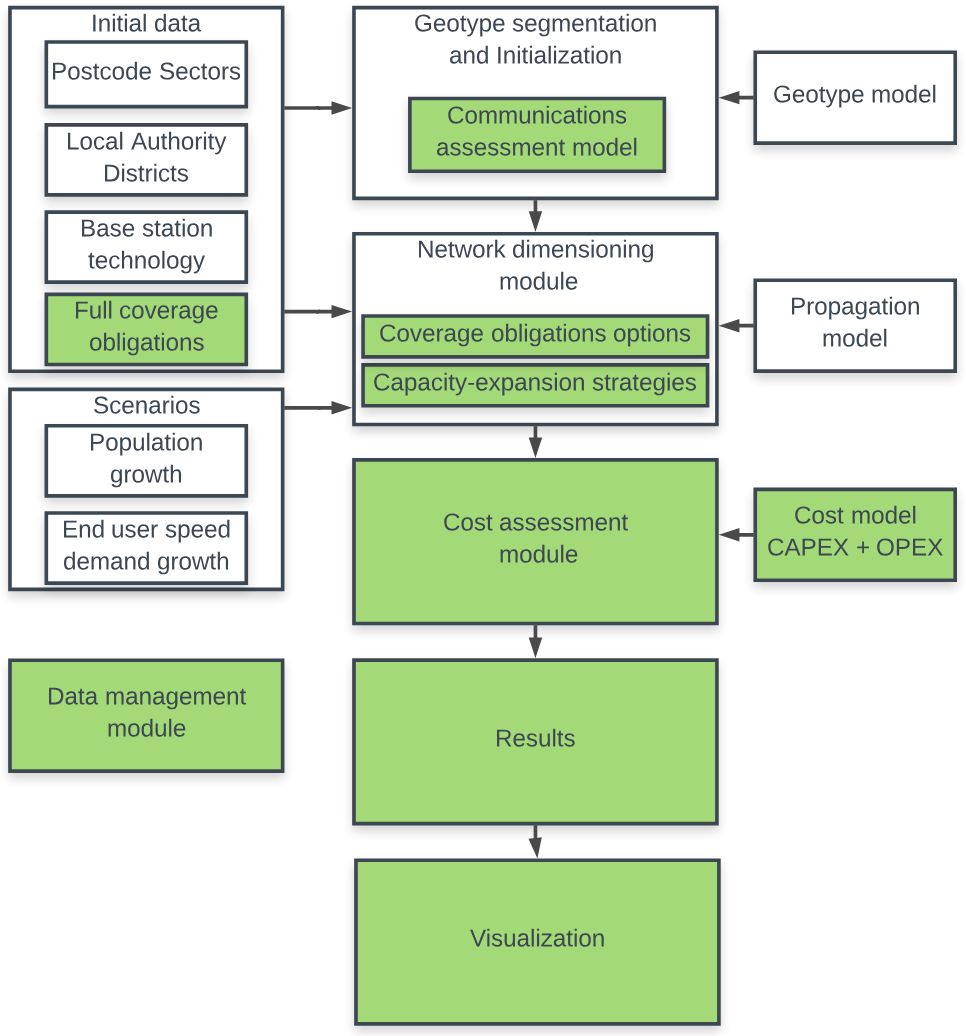
\includegraphics[width=0.95\textwidth]{./media/image28.png}
		\caption{NISMOD architecture with the new modules. Source: Author}
	\end{Center}
\end{figure}


%%%%%%%%%%%%%%%%%%%% Figure/Image No: 28 Ends here %%%%%%%%%%%%%%%%%%%%

\subsection{Coverage obligations options}
%\addcontentsline{toc}{subsection}{Coverage obligations options}
This project is aimed at defining realistic coverage obligations to test real scenarios. Coverage obligation options defined in this chapter base on the analysis presented in chapter 2 where we reviewed the content and characteristics of coverage obligations in some of the countries in Europe. The analysis was mainly focused on Spain, the UK, France, and Germany. \par

The characteristics of these coverage obligations have been extracted and condensed in the following four options: \par

\begin{itemize}
	\item \textit{«Priority areas first»} forces telecom operators to invest only in rural areas.\par

	\item \textit{«Less profitable first»} forces to invest first in the most profitable areas of each nation.\par

	\item \textit{«Only rural areas forces»} to invest in the priority areas first.\par

	\item \textit{«Nation-balanced»} forces to invest first in the less profitable areas. 
\end{itemize}\par

In addition, two more simple options have been defined to understand the rest: \textit{«Business as usual»} and \textit{«More profitable first».}\par

In this section, we define these options and how they operate. Later on, in chapter 4, we will analyze how they work in the simulation and which advantages and disadvantages they have.\par

\subsubsection*{Business as usual (No coverage obligations)}
%\addcontentsline{toc}{subsubsection}{Business as usual (No coverage obligations)}
This is, strictly speaking, not a coverage obligation option since there are no coverage obligations here. The following diagram represents all the PCDs in descending order from higher population density to lower density. As, in this case, telecom operators do not have to invest imperatively in any area, they would logically build assets first in those areas that demand more capacity than what is installed starting in those regions were investing is more profitable than others. In the diagram, the full line is red coloured because no PCD will receive more or fewer investments due to coverage obligations.



%%%%%%%%%%%%%%%%%%%% Figure/Image No: 29 starts here %%%%%%%%%%%%%%%%%%%%

\begin{figure}[H]
	\begin{Center}
		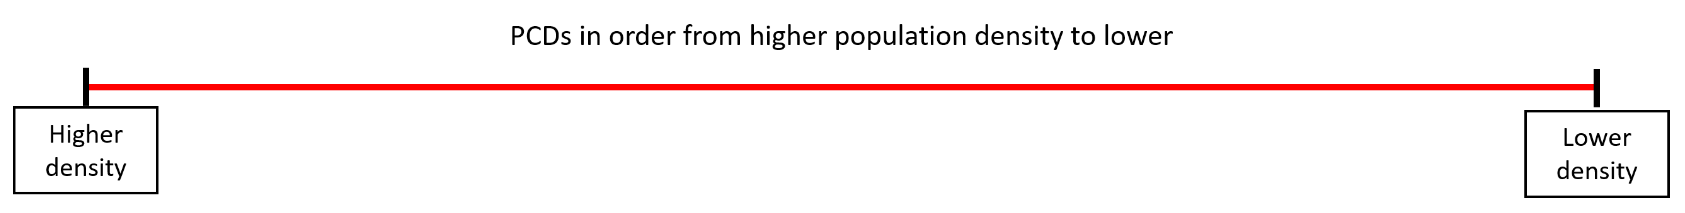
\includegraphics[width=0.95\textwidth]{./media/image29.png}
		\caption{Coverage obligations in \textit{«Business as usual»}. Source: Author}
	\end{Center}
\end{figure}


%%%%%%%%%%%%%%%%%%%% Figure/Image No: 29 Ends here %%%%%%%%%%%%%%%%%%%%


\subsubsection*{More profitable first (Original model)}
%\addcontentsline{toc}{subsubsection}{More profitable first (Original model)}
This other option is just the simple model that does have a coverage obligation, but where there is no coverage obligation compliance. This way, the telecom operator will be forced to achieve a minimum user download speed for a given year, but it will not need to do it in a specific way, technology, or band, and neither to invest in some specific areas before others. This is the behaviour of the original NISMOD project and will be used as a template to compare with the rest of them.\par

The following diagram represents the way telecom operators would probably invest if they follow this option. They would like to maximize profitability and thus, in a similar way as in the business as usual case, they would start to invest in the most densely populated PCDs until they can cover the coverage obligations in this PCD. Then they will continue investing until they reach a certain percentage of the population covered, where they will stop.



%%%%%%%%%%%%%%%%%%%% Figure/Image No: 30 starts here %%%%%%%%%%%%%%%%%%%%

\begin{figure}[H]
	\begin{Center}
		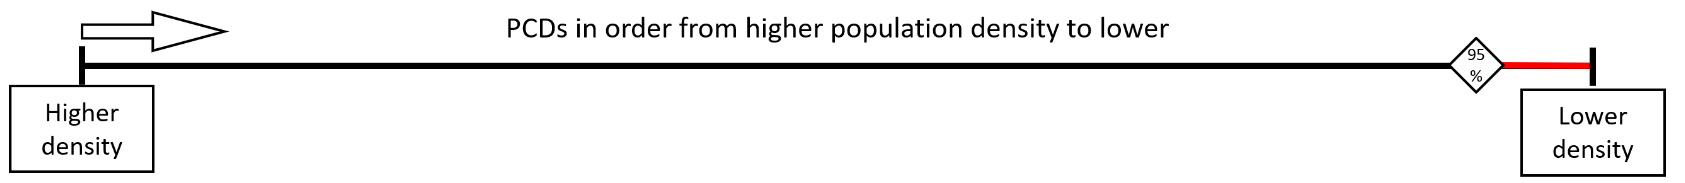
\includegraphics[width=0.95\textwidth]{./media/image30.png}
		\caption{Coverage obligations in \textit{«More profitable first»}. Source: Author}
	\end{Center}
\end{figure}


%%%%%%%%%%%%%%%%%%%% Figure/Image No: 30 Ends here %%%%%%%%%%%%%%%%%%%%


Note that the red line represents the part of the PCDs that will be left out of the coverage obligations.\par

\subsubsection*{Priority areas first (France)}
%\addcontentsline{toc}{subsubsection}{Priority areas first (France)}
This option is inspired by the coverage obligations that Arcep, the French regulator, imposed on telecom operators in France. This option tests the efficiency and the profitability of creating a priority area where telecom operators must invest first to be allowed to follow to cover the same (or a different) coverage obligation in the rest of the PCDs.\par

This thesis uses the UK’s geographic and demographic data to test all the coverage obligations in a similar scenario, so there is no list of the priority areas of the UK. As selecting the areas that are less developed in telecommunication services in the UK would not imply to have better results, the approach followed in the thesis is to select areas that sum the same population in the UK than the priority areas from France, which were 18$\%$  of the population according to Arcep. Those PCDs will be chosen beginning at the most rural PCD.\par

Once the limit is established, if telecom operators would like to maximize their profitability, they would roll out broadband services in three steps:\par

	\item Invest first starting in the limit $``$priority – non-priority$"$  covering the priority areas.\par

	\item Then, start in the most profitable PCD and continue until every PCD has their coverage obligations fulfilled.\par

	\item After that, they would be able to build more assets to increase the capacity of those PCDs that still need more investment.\par

The following diagram shows this option and allows to compare it with the previous ones. Note that in this option no minimum percentage has been defined so every postcode has to fulfil the obligations. This is completely customizable in the code, but the decision has been taken because Arcep defined a 99.6$\%$  coverage obligation in the entire territory and this option wants to check the effects that this decision will have in the costs.



%%%%%%%%%%%%%%%%%%%% Figure/Image No: 31 starts here %%%%%%%%%%%%%%%%%%%%

\begin{figure}[H]
	\begin{Center}
		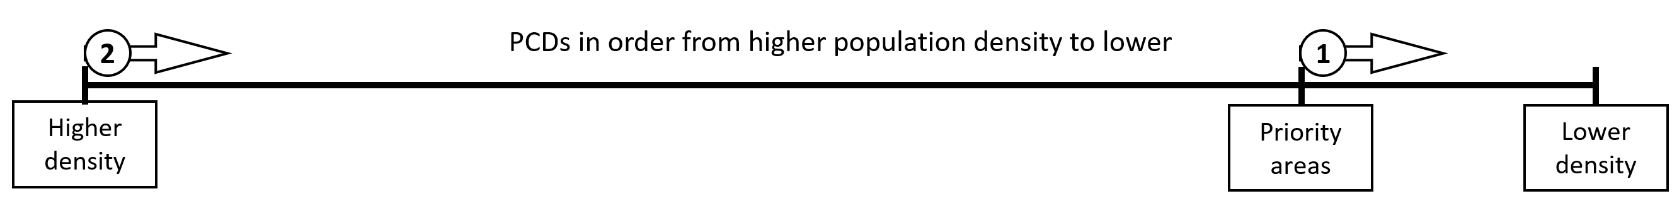
\includegraphics[width=0.95\textwidth]{./media/image31.png}
		\caption{Coverage obligations in \textit{«Priority areas first»}. Source: Author}
	\end{Center}
\end{figure}


%%%%%%%%%%%%%%%%%%%% Figure/Image No: 31 Ends here %%%%%%%%%%%%%%%%%%%%


\subsubsection*{Less profitable first (Germany)}
%\addcontentsline{toc}{subsubsection}{Less profitable first (Germany)}
This option is based on the strategy that Germany followed to set their coverage obligations. They defined four groups according to population density and only allowed telecom operators to invest in more densely populated groups if they had achieved a minimum percentage of coverage in the lower ones. This strategy is interesting because investments are not motivated by a necessity of fulfilling obligations but by their interest in investing as soon as possible in the most profitable areas.\par

For the sake of simplicity, no intermediate steps have been defined, just a global 95$\%$  of the population covered by the obligations at the end of the period. In this scenario, the normal approach of each telecom operator would be to not consider the 5$\%$  less profitable part of the population.\par

Once the 95$\%$  of the population is selected, according to this option, the telecom operator will invest in the less profitable areas and then it will continue area per area, investing in all the areas that need to improve their assets to meet the coverage obligations until they finish building assets in the most profitable one. The following diagram shows how a telecom operator should invest in the $``$Less profitable first$"$  scenario:



%%%%%%%%%%%%%%%%%%%% Figure/Image No: 32 starts here %%%%%%%%%%%%%%%%%%%%

\begin{figure}[H]
	\begin{Center}
		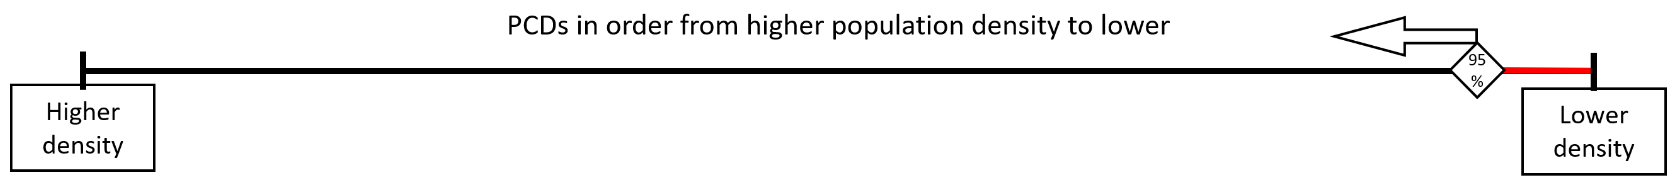
\includegraphics[width=0.95\textwidth]{./media/image32.png}
		\caption{Coverage obligations in \textit{«Less profitable first»}. Source: Author}
	\end{Center}
\end{figure}


%%%%%%%%%%%%%%%%%%%% Figure/Image No: 32 Ends here %%%%%%%%%%%%%%%%%%%%



Note that the red line represents the part of the PCDs that will not be affected by the coverage obligations.\par

\subsubsection*{Only rural areas (Spain)}
%\addcontentsline{toc}{subsubsection}{Only rural areas (Spain)}
The following option is focused on only balancing the mobile broadband gap that occurs in most of the countries between the rural and the urban and suburban areas. This option is based on the coverage obligations that Spain established for telecom operators in Spain. The interesting point of this option is that it does not enforce a coverage obligation for most of the regions, but only for those that are less populated.\par

This strategy first looks for those regions that are rural, due to their population. These are the only regions that are affected by the coverage obligation. After that, the obligation says that with only 90$\%$  of those is enough to fulfil the obligation, so following the same approach of before, it is expected that the 10$\%$  of the rural PCDs that is less populated will be excluded.\par

Of course, after fulfilling the coverage obligations, telecom operators can invest in any PCD to improve the capacity of the network and provide more download speed to their users, but this is not part of the coverage obligation.



%%%%%%%%%%%%%%%%%%%% Figure/Image No: 33 starts here %%%%%%%%%%%%%%%%%%%%

\begin{figure}[H]
	\begin{Center}
		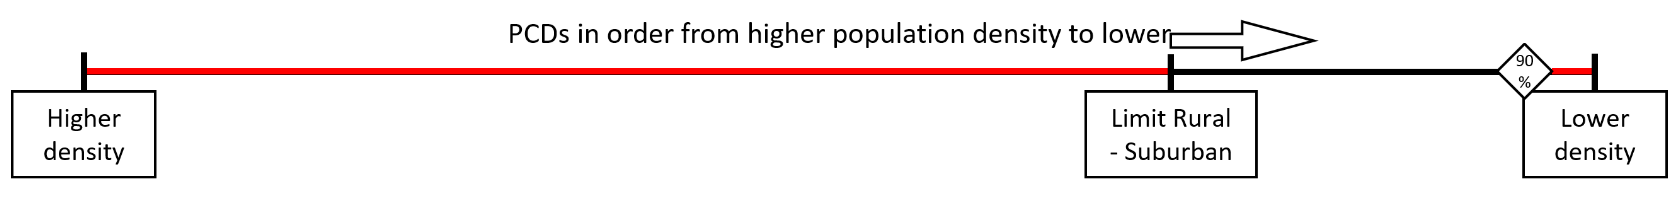
\includegraphics[width=0.95\textwidth]{./media/image33.png}
		\caption{Coverage obligations in \textit{«Only rural areas»}. Source: Author}
	\end{Center}
\end{figure}


%%%%%%%%%%%%%%%%%%%% Figure/Image No: 33 Ends here %%%%%%%%%%%%%%%%%%%%


\subsubsection*{Nation-balanced (The United Kingdom)}
%\addcontentsline{toc}{subsubsection}{Nation-balanced (The United Kingdom)}
This is the last option proposed in this project and is related to the coverage obligation imposed in the UK. The UK comprises four nations with different characteristics in the telecommunications field. First, England is by far the most populated and also contains most of the densely populated areas. On the contrary, regions like Scotland are more rural, have more uninhabited areas and more mountainous terrain, which make most of their PCDs less profitable to invest in. For that reason, Ofcom, the British policymaker, decided to split the coverage obligations into the four countries, so that telecom operators invest in all the countries equally independently of the profitability of investing more in some than in others.\par

This option is like the $``$More profitable first$"$  option but split into countries. The algorithm still checks all the PCDs in order from more profitable to less but keeps the percentage of people that are covered in each country. When one country is completely covered, the algorithm continues checking but no more PCDs from this country can be considered.



%%%%%%%%%%%%%%%%%%%% Figure/Image No: 34 starts here %%%%%%%%%%%%%%%%%%%%

\begin{figure}[H]
	\begin{Center}
		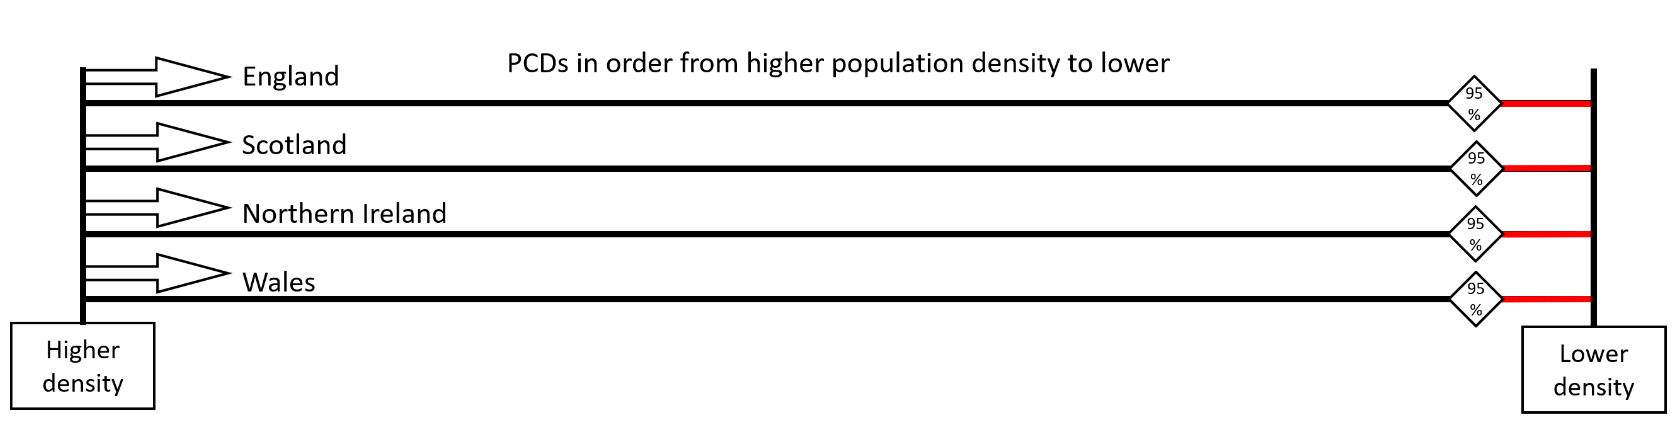
\includegraphics[width=0.95\textwidth]{./media/image34.png}
		\caption{Coverage obligations in \textit{«Nation-balanced»}. Source: Author}
	\end{Center}
\end{figure}


%%%%%%%%%%%%%%%%%%%% Figure/Image No: 34 Ends here %%%%%%%%%%%%%%%%%%%%

\subsection{Initial Data}
Two main improvements have been undertaken in this part of the code: the implementation of the Data Management Structure and the code to define coverage obligations. Nonetheless, other parts of the code have been modified and refined such as the new simulation options (To test new scenarios) and the new parameters of the end-user speed (Which is loaded from a file in this step).\par

\subsubsection*{Data management structure}
%\addcontentsline{toc}{subsubsection}{Data management structure}
The data management structure is a module called ‘\textit{results.py’} that is initialized at the beginning of the execution and stores all the information that the user might want to print at the end. It is just a class called Results that contains several sets of Chart subclasses for each simulation option. Chart subclasses are classes that store information of each PCD and are so related to each of the charts that are drawn from the execution. Some columns such as the PCD ID and the PCD population are initialized at the beginning and after that, each valuable output is picked and copied to the structure. When the Visualization module is called, it looks for all these classes, takes the information and manipulates it to print plots, maps and csv. \par

It also allows storing some environment values that will remain unchangeable during a great part of the execution of the code. It stores the output paths of the plots and maps modules, the total population of the country to reduce the time-consuming task that is to add the population of 9,000 PCDs every time the code needs to know the total population of the country, it stores the maps file paths of the images that will be added to gifs and it also stores all the information of the coverage obligation that is set at any time. \par

In the end, this module acts as a big bundle that allows having everything ready to use, saving time and resources.\par

\subsubsection*{Coverage obligations structure}
%\addcontentsline{toc}{subsubsection}{Coverage obligations structure}
In order to make coverage obligations completely customizable and adjustable, they are defined in a dictionary at the beginning of the execution and loaded into the Data management structure, so that the information about the current coverage obligation can be checked at any one moment.\par

These are the parameters that I have selected to describe a coverage obligation in this thesis: \par

\begin{enumerate}
	\item The coverage id, name, and description to have an unambiguous identifier of the obligation.\par

	\item The population limit, defined with a Boolean and a number limit, which defines the maximum population of the PCDs that are subject to the coverage obligations. \par

	\item The priority deployment that determines the percentage of the population whose PCDs will be part of the priority deployment areas. In this case, only France will have a number different from 0, but any coverage option could implement this strategy.\par

	\item The budget limits Boolean defines if this coverage obligation option is limited by the budget estimated for each telecom operator or not. The estimated budget amounts to 2 billion pounds multiplied by the market share (30$\%$  in this case) per year. This option will be used in the results chapter to check how much money would be necessary to fulfil the coverage obligations in case that not everybody can be covered with the estimated budget.\par

	\item The descending order parameter defines if the telecom operator should start investing in the more or the less profitable areas first. This Boolean is always true, except in the $``$Less profitable first$"$  option, where it is false, which inverts the order of investment decision of the PCDs.\par

	\item Invest by demand is a parameter that allows setting if, after investing to meet the coverage obligations, the telecom operator can continue investing money to build assets that can increase the capacity of the network to meet the demand in those PCDs where it is higher than the coverage obligations.\par

	\item The percentage covered is the minimum percentage of the population that the policymaker requires the telecom operators to cover. It depends on the coverage obligation and in the case of the $``$Only rural areas$"$  option, the percentage applies only to the rural areas, not to the total of PCDs.\par

	\item Finally, coverage\_obligation is a sub-dictionary that allows setting several end-user speeds depending on the requirements of the policymaker. There are three possible levels: Low, baseline and high and in this example the values are 2, 5 and 8 Mbps.
\end{enumerate}
\begin{lstlisting}[language=Bash]
'cov_ob_1': {
        'name': 'Coverage Obligation 1',
        'description': 'Original coverage obligation',
        'population_limit_boolean': False,
        'population_limit': None,
        'deploiement_prioritaire': 0,
        'budget_limit': True,
        'descending_order': True,
        'invest_by_demand': True,
        'percentage_covered': 1,
        'coverage_obligation': {
                'low': 2,
                'baseline': 5,
                'high': 8
        },
    }
\end{lstlisting}

\subsubsection*{Simulation options}
%\addcontentsline{toc}{subsubsection}{Simulation options}
Two new options have been added to the model to be able to test all the possibilities of the code and both are related to the coverage obligations:\par

	\item \textit{coverage\_obligation\_type} is the variable that specifies the option set for this execution of the code. It may take one of the values defined in the coverage obligations structure.\par

	\item \textit{coverage\_speed\_scenario }is the degree of intensity of the coverage obligation set by the policymaker. \par

\subsection{Geotype segmentation and initialization}
The only change in this module is in the way the code sorts each PCD into geotypes.\par

\subsubsection*{Change of rural-suburban-urban}
%\addcontentsline{toc}{subsubsection}{Change of rural-suburban-urban}
The function that categorized the code in the previous code had a bug that only set as rural areas those with 0 or less population density and urban areas from 782 inhabitants per km\textsuperscript{2}. This thesis raises the population ranges and categorizes areas from 0 to 782 inhabitants per km\textsuperscript{2} as rural, from 782 to 7,959 inhabitants per km\textsuperscript{2} as suburban and from 7,959 inhabitants on as urban.\par

After making those changes, an issue arises since some PCDs that are now categorized as rural, but have a high population density (For example, 600 inhabitants per km\textsuperscript{2}) cannot satisfy the demand. This is because the propagation diagrams estimate less network capacity for rural areas than for suburban geotypes. It is not a problem or a bug by itself, it just modifies considerably the predictions made based on the previous behaviour of the project.\par

\subsection{Scenario projections}
Changing the population and end-user projection is out of the scope of the thesis because this is part of the NISMOD project and not of the digital comms submodule, but this Thesis presents an enhancement of the end-user speed demand calculation.\par

\subsubsection*{Demand in Speed or Download cap}
%\addcontentsline{toc}{subsubsection}{Demand in Speed or Download cap}
The original project calculates the end-user speed demand in downloaded GB per month and then transforms this real measured demand to Mbps multiplying it by 1024 MB in 1 GB, 8 bits in a byte, 30 days in a month, percentage\_in\_busy\_hour (which is 7.5$\%$  of the traffic of the day) and 3600 to convert from hours to seconds.\par


\begin{Center}
\begin{multline*}
Demand \_ in \_ mbps =Demand \_ in \_ GB \ \ast \ 1024 \ \ast 8 \ast \\
 Traffic \_ in \_ busy \_ hour \ / 30 \ / 3600
\end{multline}
\end{Center}\par

The problem in this estimation is that user satisfaction is not only based in the amount of data the user can download during the day but in the maximum peak speed, the user can obtain from the network. Users will have a better user-experience if both demands are covered.\par

For this purpose, the code has been modified to implement both comparisons and the demand is the more restrictive value from the demand by speed and demand by download capacity.\par

In the newest version of the code, the user can create a csv file to introduce the evolution of the user demand in Mbps for each year until 2030 for three different scenarios: low demand, baseline demand, and high.\par

\subsection{Network dimensioning module}
This is the module that suffered more technical changes since now the model behaves quite different as it does at the beginning of the thesis. There are two big changes in this module: \par

\begin{itemize}
	\item The implementation of a new strategy called 700 MHz densification, that allows creating more assets for 700 MHz when the existing ones are already upgraded to 700 MHz until the maximum capacity of the network is reached (The maximum capacity is calculated using the propagation model).\par

	\item The creation of a more complex way of organizing the PCDs to comply with the obligations.
\end{itemize}\par

This module consists of several steps that enable to decide the interventions of all the PCDs for the whole year:\par

\begin{enumerate}
	\item Once a new year starts, this module is called to select those PCDs that, according to the coverage obligation option should meet the obligations, and orders them according to the option.\par

	\item It removes from the list those PCDs that already met the coverage obligation, thanks to the assets that were already installed before the execution or because they were built in a previous year in the simulation.\par

	\item For each PCD, it checks which are the interventions that are allowed according to the capacity expansion strategy and builds new assets in a given order. If all the interventions are allowed, the order is the following:\par

\setlength{\parskip}{7.92pt}
\begin{enumerate}
	\item First, it checks if more LTE upgrades are possible.\par

	\item If the capacity is not enough, it also integrates the 700 MHz band (This integration can be just upgrading the current assets or building new ones, it depends on the coverage obligation option).\par

	\item It integrates the 3,500 MHz band.\par

	\item The last resource is to build small cells.\par


\end{enumerate}
	\item This loop continues checking each PCD until there is no more budget for the given year or when the full list of PCD meets the coverage obligations and there is more budget.\par

	\item {\fontsize{11pt}{13.2pt}\selectfont In case that there is no more budget, the execution ends. In the other case, the code lists all the PCDs from more densely populated to less, removes those whose capacity margin is positive (Because they do not need more investment) and repeats the previous steps but with this list until there is no more budget.\par}
\end{enumerate}\par

Finally, all the new assets are stored and loaded into the system model to use them in the following year.\par

\setlength{\parskip}{8.04pt}
\subsubsection*{Coverage obligations}
%\addcontentsline{toc}{subsubsection}{Coverage obligations}
As seen, the network dimensioning module has four steps: select PCDs for the coverage obligations, invest, select all the PCDs that have a capacity deficit and invest to increase their network capacity.\par

The code modification needed for the coverage obligations feature modifies the first step. Based on the coverage obligation id and parameters, the code selects and orders PCDs in a specific way. The code also orders the visualization module PCDs in the same way, so they are displayed correctly. \par

\subsubsection*{700MHz Densification}
%\addcontentsline{toc}{subsubsection}{700MHz Densification}
The 700 MHz densification is the new intervention designed in the thesis and it is implemented in this module. In this work, it only belongs to the macrocell\_only\_700 capacity expansion strategy which only allows the 700 MHz densification intervention when it is enabled, but it is configurable in the initialization structures.\par

As 700 MHz could be built using the already installed assets or standalone installations, this intervention functions as a combination of the behaviour of the normal 700 MHz and the small cells interventions. When the network dimensioning module selects one PCD to invest and this intervention is triggered, it checks how many assets have LTE and 700 MHz carriers. If there are assets that still have no 700 MHz carrier but have the LTE bands available, the intervention just builds a new 700 MHz carrier on the asset. If there are no more assets without 700, it deploys a new base station with 700 MHz. Costs of both scenarios are different and calculated based on the costings tables.\par

\subsection{Cost assessment module}
Costs are calculated in the same way as in the original model. After the execution of all the interventions, the full list of new assets is checked by the cost assessment module and the total cost of the year is calculated.\par

\subsubsection*{Cost model}
%\addcontentsline{toc}{subsubsection}{Cost model}
The cost model has been updated to include the new intervention costs. In case of building a new carrier in an existing installation, the cost is the same as in the 700MHz intervention: CAPEX is the cost of installing an additional carrier on the current base station, which is £15,000, and OPEX is £1,800. Therefore, the total cost discounted to the present value is £50,917.\par

For new installations, costs are like deploying a new base station for LTE, despite 700MHz would be the only carrier available. In this case, CAPEX is the cost of deploying two multicarrier base stations (2 x £40,900) plus the cost of the civil works (£18,000) and OPEX is £3,898 per year. The total cost discounted to the present value is £142,446. For a deeper explanation of costs, please refer to the Cost assessment module section of the original project or \cite{3-03}.\par

\subsection{Model results}
While deciding the interventions and calculating costs, the program stores and computes some key values of the system, so that the visualization model can store it later. Apart from storing values of costs and capacity margin, which was already implemented and explained in the previous chapter, it calculates (I) the percentage of population in each PCD that has the minimum capacity that the coverage obligation defines, (II) the number of assets that are upgraded or built depending on the technology per PCD, (III) values of population, (IV) demand and capacity per PCD and (V) global values calculated after deciding all the interventions of a simulation.\par

It is also capable of aggregating all of this data to the LAD level. Some values can be added directly, such as population and costs, but others, such as the percentage of population covered or the capacity margin not. Therefore, these parameters are aggregated weighted by population.\par

All the values are stored in the Results module, which is initialized in the $``$Initial Data$"$  step and then the rest of parameters are added whenever they are available. The results module is just a class that contains several dictionaries of classes that store all the values. Each set is different since they contain different types of subclasses, each of them defined to store information of one specific value. This way, despite some information, could be stored redundantly, it allows to expand the capabilities faster because creating a new table calculating new values means simply creating a new set and previous information is not altered.\par

\subsubsection*{Population, demand, and capacity}
%\addcontentsline{toc}{subsubsection}{Population, demand, and capacity}
In previous versions of the code, these were intermediate values to decide interventions and to calculate demand and capacity, but their evolution was not stored. Now, the visualization module shows the change of them over time and generates plots, maps, and csv with their values. The following map, for example, shows the population per PCD at the beginning of the execution, in 2020. It can be visualised over the entire period under study.



%%%%%%%%%%%%%%%%%%%% Figure/Image No: 35 starts here %%%%%%%%%%%%%%%%%%%%

\begin{figure}[H]
	\begin{Center}
		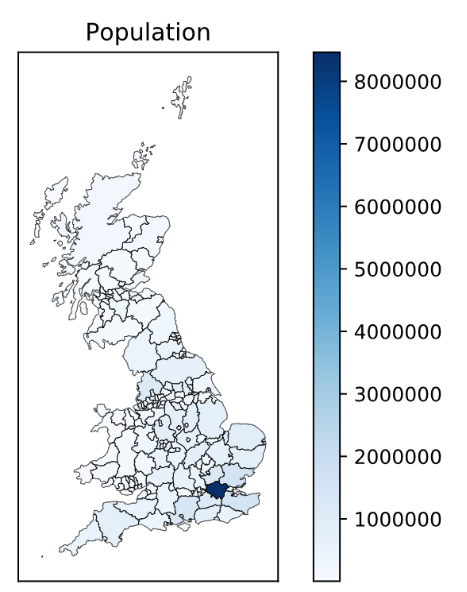
\includegraphics[width=0.70\textwidth]{./media/image35.png}
		\caption{Population distribution in the UK. Source: Author}
	\end{Center}
\end{figure}


%%%%%%%%%%%%%%%%%%%% Figure/Image No: 35 Ends here %%%%%%%%%%%%%%%%%%%%



\subsubsection*{Technology upgrades}
%\addcontentsline{toc}{subsubsection}{Technology upgrades}
A similar situation occurs with the number of sites built or upgraded per technology per year. The code now stores all the information about technology upgrades and calculates the number of upgrades that occurred per year in each PCD. The visualization module outputs maps, csv files and figures with the evolution.\par

For example, the following coloured map represents the number of technology upgrades made in the execution of the scenario of medium growth of population and user-speed demand, with the $``$More profitable first$"$  coverage obligation option that enforces 2 Mbps and with the capacity expansion strategy that only allows building 700 MHz cells:



%%%%%%%%%%%%%%%%%%%% Figure/Image No: 36 starts here %%%%%%%%%%%%%%%%%%%%

\begin{figure}[H]
	\begin{Center}
		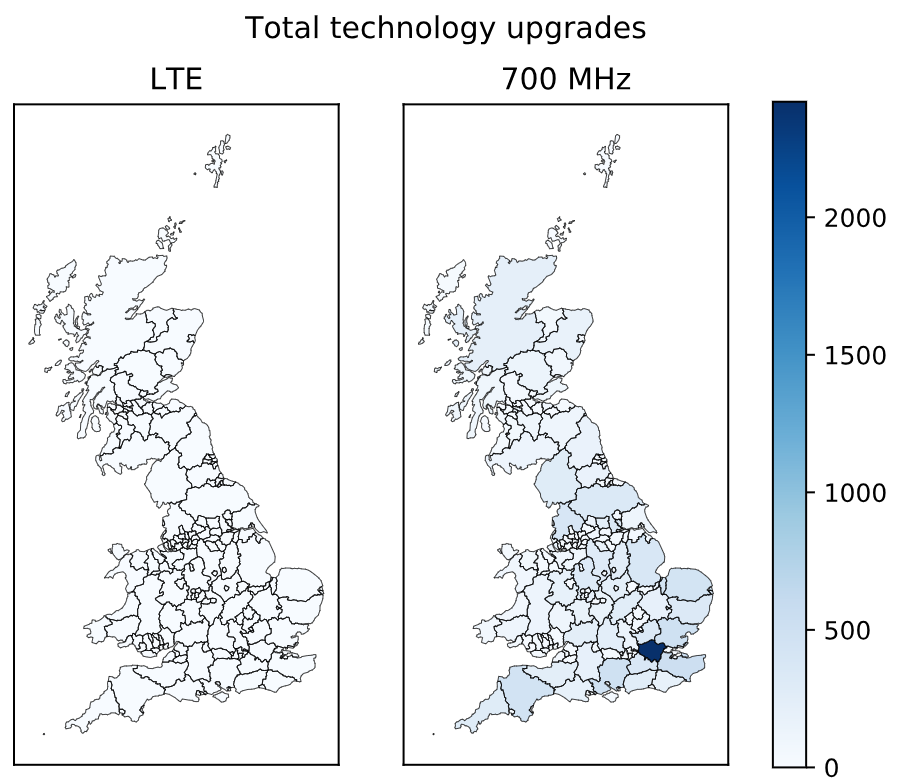
\includegraphics[width=0.85\textwidth]{./media/image36.png}
		\caption{Technology upgrades with \textit{«700MHz densification}. Source: Author}
	\end{Center}
\end{figure}


%%%%%%%%%%%%%%%%%%%% Figure/Image No: 36 Ends here %%%%%%%%%%%%%%%%%%%%


\subsubsection*{Population covered}
%\addcontentsline{toc}{subsubsection}{Population covered}
Population covered is another output of the project. When a year ends, the system computes the percentage of the population covered as the result of the division of the capacity by the download speed demand in each PCD. The result is capped to one since the population covered cannot be more than 100$\%$ .\par

The following coloured maps represent the population covered per year in the execution of the scenario of medium growth of population and user-speed demand, with the $``$More profitable first$"$  coverage obligation option that enforces 2 Mbps and with the capacity expansion strategy that only allows building 700 MHz cells:



%%%%%%%%%%%%%%%%%%%% Figure/Image No: 37 starts here %%%%%%%%%%%%%%%%%%%%

\begin{figure}[H]
	\begin{Center}
		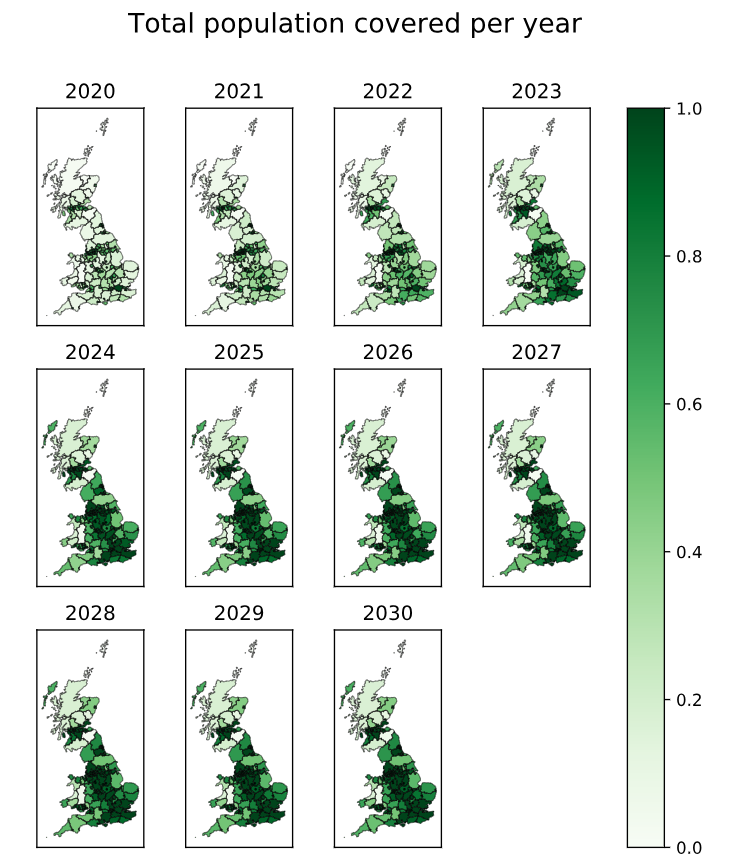
\includegraphics[width=0.95\textwidth]{./media/image37.png}
		\caption{Example of the evolution of the percentage of population covered with the \textit{«700MHz densification} capacity expansion strategy. Source: Author}
	\end{Center}
\end{figure}


%%%%%%%%%%%%%%%%%%%% Figure/Image No: 37 Ends here %%%%%%%%%%%%%%%%%%%%


\subsubsection*{How to aggregate capacity and demand values}
%\addcontentsline{toc}{subsubsection}{How to aggregate capacity and demand values}
Aggregating values from PCDs to LADs is not always as simple as just adding values. Aggregating costs and technology upgrades can be made just by adding values of each PCD. However, percentages of the population covered cannot be aggregated but weighted according to a specific factor, such as population or area. Since covered obligations are defined based on population, these values are weighted by population. \par


 \[ \% Population_{LAD}=\frac{ \sum _{1}^{N}Population_{PCD-i}  \times  \% Population_{PCD-i}}{ \sum _{1}^{N}Population_{PCD-i} } \] \par
	
	where N is the number of PCDs.

The capacity margin is expressed in Mbps/km\textsuperscript{2} and cannot be aggregated directly because is a relative measure, not an absolute value of capacity margin. This way, it must be weighted, as well. The following chart represents a LAD that contains 9 PCDs. Since coverage obligations are population oriented, if PCD 1 has 90$\%$  of the population and the rest is distributed among the others, the capacity margin of the PCD 1 has to weight 90$\%$  of the total calculus of the capacity margin. The following formula is used.



%%%%%%%%%%%%%%%%%%%% Table No: 7 starts here %%%%%%%%%%%%%%%%%%%%

\begin{table}[H]
\begin{center}
\begin{tabular}{ |c|c|c| } 
\hline
{\cellcolor[HTML]{2F5496}\Centering 1} & 2 & 3 \\ 
\hline
4 & 5 & 6 \\ 
\hline
7 & 8 & 9 \\ 
\hline
\end{tabular}
\end{center}
\end{table}


%\begin{table}[H]
 			%\centering
%\begin{tabular}{p{0.1in}p{0.1in}p{0.1in}}
%\hline
%%row no:1
%\multicolumn{1}{|p{0.1in}}{\cellcolor[HTML]{2F5496}\Centering 1} & 
%\multicolumn{1}{|p{0.1in}}{\cellcolor[HTML]{D9E2F3}\Centering 2} & 
%\multicolumn{1}{|p{0.1in}|}{\cellcolor[HTML]{D9E2F3}\Centering 3} \\
%\hhline{---}
%%row no:2
%\multicolumn{1}{|p{0.1in}}{\cellcolor[HTML]{D9E2F3}\Centering 4} & 
%\multicolumn{1}{|p{0.1in}}{\cellcolor[HTML]{D9E2F3}\Centering 5} & 
%\multicolumn{1}{|p{0.1in}|}{\cellcolor[HTML]{D9E2F3}\Centering 6} \\
%\hhline{---}
%%row no:3
%\multicolumn{1}{|p{0.1in}}{\cellcolor[HTML]{D9E2F3}\Centering 7} & 
%\multicolumn{1}{|p{0.1in}}{\cellcolor[HTML]{D9E2F3}\Centering 8} & 
%\multicolumn{1}{|p{0.1in}|}{\cellcolor[HTML]{D9E2F3}\Centering 9} \\
%\hhline{---}
%
%\end{tabular}
 %\end{table}


%%%%%%%%%%%%%%%%%%%% Table No: 7 ends here %%%%%%%%%%%%%%%%%%%%


 \[ Capacity\_ margin_{LAD}=\frac{ \sum _{1}^{N}Population_{PCD-i}  \times  Capacity\_ margin_{PCD-i}}{ \sum _{1}^{N}Population_{PCD-i} } \] \par
	
	where N is the number of PCDs.

\subsubsection*{Global variables}
%\addcontentsline{toc}{subsubsection}{Global variables}
Finally, some global values are also calculated after each simulation ends, and results of several simulations are compared to see the advantages or disadvantages of each of them. The values stored are the population, investment cost, population covered, number of PCDs covered and capacity margin per year. The array also stores if the model had enough budget to invest by demand.\par

The following diagram represents an example of the cost of incrementing the percentage of population covered for a given coverage obligation. The results and analysis section cover this in greater detail.



%%%%%%%%%%%%%%%%%%%% Figure/Image No: 38 starts here %%%%%%%%%%%%%%%%%%%%

\begin{figure}[H]
	\begin{Center}
		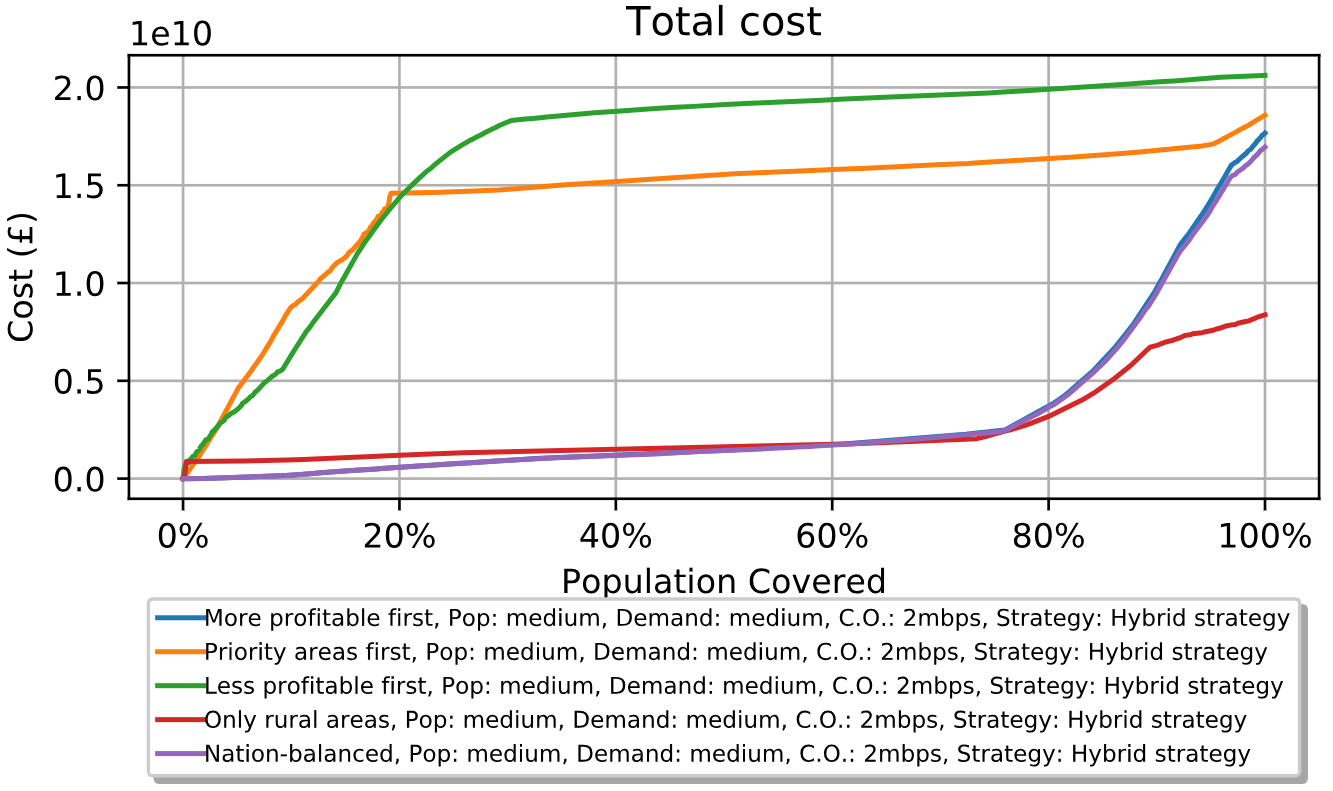
\includegraphics[width=0.95\textwidth]{./media/image38.png}
		\caption{Example of the investment with the \textit{«700MHz densification} capacity expansion strategy.Source: Author}
	\end{Center}
\end{figure}


%%%%%%%%%%%%%%%%%%%% Figure/Image No: 38 Ends here %%%%%%%%%%%%%%%%%%%%

\subsection{Visualization}
Once all the results are calculated and stored in the Results bundle, the code calls some functions of the Save Data module, which acts as a hub that takes the interesting results and represents them as csv, maps, plots, histograms or gifs. This functionality is completely new to the project and it is the tool that has been used to create all the diagrams and images of the results chapter.\par

\subsubsection*{Plots}
%\addcontentsline{toc}{subsubsection}{Plots}
Plots are the best way of comparing the output between different simulations of the project since they have more accuracy than maps (That do not have enough definition to see the differences between rural and urban areas), but they allow to see the whole picture of the situation (CSV files are so big that they are mainly used to check specific values). All the plots are allocated under the Outputs folder and inside the $``$figures$"$  folder. For a given simulation, the main plots drawn in the code are the following: \par

\begin{enumerate}[label*=\arabic*.]
	\item Aggregation of the investment in each PCD for all the years and calculation of the cost in pounds of increasing the population covered percentage. These plots start with the code 1\_1\_cost.\par

	\item Representation of the evolution of the investment through PCDs over the years. It allows seeing how the main part of the investment costs move from left to right, which means that the project invests in the same order of the list of PCDs, which depends on the coverage option. These plots start with the code 1\_2\_cost\_per\_year\_all.\par

	\item Representation of the technology upgrades through PCDs along the years. It allows seeing how the main part of the investment costs move from left to right, which means that the project invests in the same order of the list of PCDs, which depends on the coverage option. These plots start with the code 3\_1\_tech\_upgrades\_per\_year\_all.\par

	\item Representation of the capacity (Mbps per km\textsuperscript{2}) over the years in each PCD. These plots start with the code 4\_1\_capacity.\par

	\item Representation of the demand (Mbps per km\textsuperscript{2}) over the years in each PCD. These plots start with the code 4\_2\_demand.
\end{enumerate}\par

Despite all these representations study the implications of a single simulation, this module creates charts for comparing several of them, as well. There are three main plots:\par

\begin{enumerate}[label*=\arabic*.]
	\item Aggregation of the investment in each PCD for all the years and calculation of the cost in pounds of increasing the population covered percentage. This plot is under the summary folder and named \\
	1\_cost\_comparison\_per\_strategy.\par

	\item Comparison of the population covered per year and simulation option. This plot is under the summary folder and named \\
	2\_population\_covered\_per\_strategy.\par

	\item Comparison of the capacity margin per year and simulation option. This plot is under the summary folder and named \\
	3\_capacity\_margin\_per\_strategy.
\end{enumerate}\par

\subsubsection*{Histograms}
%\addcontentsline{toc}{subsubsection}{Histograms}
The main objective of the coverage obligations in most of the countries studied in chapter 2 is to reduce the end-user speed gap between the urban and the rural areas of the country. Studying the distribution of the capacity margin among all the PCDs allows the stakeholders to know the percentage of the population and the regions that have less capacity than the one enforced by the coverage obligation. The following chart shows an example of a histogram. In this case, the simulation represents the scenario of medium growth of population and user-speed demand, with the $``$Less profitable first$"$  coverage obligation option that enforces 2 Mbps and with the capacity expansion strategy that allows upgrading existing assets with LTE, 700MHz, 3,500 MHz and building small cells.



%%%%%%%%%%%%%%%%%%%% Figure/Image No: 39 starts here %%%%%%%%%%%%%%%%%%%%

\begin{figure}[H]
	\begin{Center}
		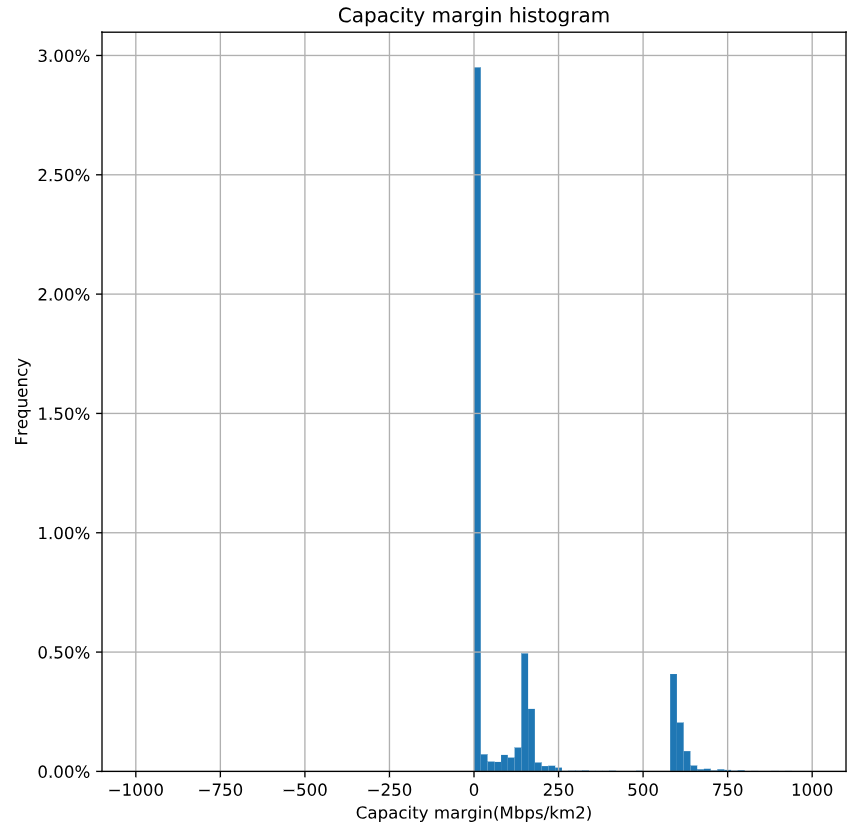
\includegraphics[width=0.95\textwidth]{./media/image39.png}
		\caption{Example of an histogram of the capacity margin per PCD with the \textit{«700MHz densification} capacity expansion strategy. Source: Author}
	\end{Center}
\end{figure}


%%%%%%%%%%%%%%%%%%%% Figure/Image No: 39 Ends here %%%%%%%%%%%%%%%%%%%%

\subsubsection*{Csv files}
%\addcontentsline{toc}{subsubsection}{Csv files}
Csv files store all the information related to the project. The advantage of this type of format is that they store the exact value of the outputs and allow to compare them with more detail than maps, plots or diagrams. There are two types of csv: Those that start with the code \textit{lad\_} refer to information represented in maps, the ones that start with the suffix \textit{pcd\_} contain information related to plots and histograms. \par

\subsubsection*{Maps}
%\addcontentsline{toc}{subsubsection}{Maps}
Maps represent outputs printed over the map of the UK and are drawn using the plot and fill functions of the matplotlib library. The UK shape is loaded from a shapefile stored in the inputs folder and can be replaced by the shape of other countries only if the PCDs and LADs are correctly modified. As it has been explained before, results have less level of detail since maps only have 174 regions. Several maps are painted automatically when the visualization module runs:\par

\begin{enumerate}
	\item Initial population and population density.\par

	\item Investment cost per LAD.\par

	\item Evolution of the cost per year.\par

	\item Evolution of the capacity margin per year.\par

	\item The number of technology upgrades per LAD.\par

	\item Evolution of the capacity per year.\par

	\item Evolution of the demand per year.\par

	\item Evolution of the population covered per year.
\end{enumerate}\par

Therefore, there are two main types of showing information in maps: standalone maps that aggregate outputs of all the years, and sprites of the situation every year.\par

\subsubsection*{Gifs}
%\addcontentsline{toc}{subsubsection}{Gifs}
Finally, the project also allows creating gifs from the images of the visualization model. The tool allows to create gifs of every value of the project, but it is focused in gifs that show the evolution of parameters such as the coverage obligation over the years, and to compare the differences between the coverage obligation resultant from different coverage obligation options and simulations.\par
